% Options for packages loaded elsewhere
\PassOptionsToPackage{unicode}{hyperref}
\PassOptionsToPackage{hyphens}{url}
%
\documentclass[
]{article}
\usepackage{lmodern}
\usepackage{amssymb,amsmath}
\usepackage{ifxetex,ifluatex}
\ifnum 0\ifxetex 1\fi\ifluatex 1\fi=0 % if pdftex
  \usepackage[T1]{fontenc}
  \usepackage[utf8]{inputenc}
  \usepackage{textcomp} % provide euro and other symbols
\else % if luatex or xetex
  \usepackage{unicode-math}
  \defaultfontfeatures{Scale=MatchLowercase}
  \defaultfontfeatures[\rmfamily]{Ligatures=TeX,Scale=1}
\fi
% Use upquote if available, for straight quotes in verbatim environments
\IfFileExists{upquote.sty}{\usepackage{upquote}}{}
\IfFileExists{microtype.sty}{% use microtype if available
  \usepackage[]{microtype}
  \UseMicrotypeSet[protrusion]{basicmath} % disable protrusion for tt fonts
}{}
\makeatletter
\@ifundefined{KOMAClassName}{% if non-KOMA class
  \IfFileExists{parskip.sty}{%
    \usepackage{parskip}
  }{% else
    \setlength{\parindent}{0pt}
    \setlength{\parskip}{6pt plus 2pt minus 1pt}}
}{% if KOMA class
  \KOMAoptions{parskip=half}}
\makeatother
\usepackage{xcolor}
\IfFileExists{xurl.sty}{\usepackage{xurl}}{} % add URL line breaks if available
\IfFileExists{bookmark.sty}{\usepackage{bookmark}}{\usepackage{hyperref}}
\hypersetup{
  pdftitle={Data Visualization with ggplot2 PDF version},
  pdfauthor={Data Carpentry contributors \& Montana State University R Workshops Team},
  hidelinks,
  pdfcreator={LaTeX via pandoc}}
\urlstyle{same} % disable monospaced font for URLs
\usepackage[margin=1in]{geometry}
\usepackage{color}
\usepackage{fancyvrb}
\newcommand{\VerbBar}{|}
\newcommand{\VERB}{\Verb[commandchars=\\\{\}]}
\DefineVerbatimEnvironment{Highlighting}{Verbatim}{commandchars=\\\{\}}
% Add ',fontsize=\small' for more characters per line
\usepackage{framed}
\definecolor{shadecolor}{RGB}{248,248,248}
\newenvironment{Shaded}{\begin{snugshade}}{\end{snugshade}}
\newcommand{\AlertTok}[1]{\textcolor[rgb]{0.94,0.16,0.16}{#1}}
\newcommand{\AnnotationTok}[1]{\textcolor[rgb]{0.56,0.35,0.01}{\textbf{\textit{#1}}}}
\newcommand{\AttributeTok}[1]{\textcolor[rgb]{0.77,0.63,0.00}{#1}}
\newcommand{\BaseNTok}[1]{\textcolor[rgb]{0.00,0.00,0.81}{#1}}
\newcommand{\BuiltInTok}[1]{#1}
\newcommand{\CharTok}[1]{\textcolor[rgb]{0.31,0.60,0.02}{#1}}
\newcommand{\CommentTok}[1]{\textcolor[rgb]{0.56,0.35,0.01}{\textit{#1}}}
\newcommand{\CommentVarTok}[1]{\textcolor[rgb]{0.56,0.35,0.01}{\textbf{\textit{#1}}}}
\newcommand{\ConstantTok}[1]{\textcolor[rgb]{0.00,0.00,0.00}{#1}}
\newcommand{\ControlFlowTok}[1]{\textcolor[rgb]{0.13,0.29,0.53}{\textbf{#1}}}
\newcommand{\DataTypeTok}[1]{\textcolor[rgb]{0.13,0.29,0.53}{#1}}
\newcommand{\DecValTok}[1]{\textcolor[rgb]{0.00,0.00,0.81}{#1}}
\newcommand{\DocumentationTok}[1]{\textcolor[rgb]{0.56,0.35,0.01}{\textbf{\textit{#1}}}}
\newcommand{\ErrorTok}[1]{\textcolor[rgb]{0.64,0.00,0.00}{\textbf{#1}}}
\newcommand{\ExtensionTok}[1]{#1}
\newcommand{\FloatTok}[1]{\textcolor[rgb]{0.00,0.00,0.81}{#1}}
\newcommand{\FunctionTok}[1]{\textcolor[rgb]{0.00,0.00,0.00}{#1}}
\newcommand{\ImportTok}[1]{#1}
\newcommand{\InformationTok}[1]{\textcolor[rgb]{0.56,0.35,0.01}{\textbf{\textit{#1}}}}
\newcommand{\KeywordTok}[1]{\textcolor[rgb]{0.13,0.29,0.53}{\textbf{#1}}}
\newcommand{\NormalTok}[1]{#1}
\newcommand{\OperatorTok}[1]{\textcolor[rgb]{0.81,0.36,0.00}{\textbf{#1}}}
\newcommand{\OtherTok}[1]{\textcolor[rgb]{0.56,0.35,0.01}{#1}}
\newcommand{\PreprocessorTok}[1]{\textcolor[rgb]{0.56,0.35,0.01}{\textit{#1}}}
\newcommand{\RegionMarkerTok}[1]{#1}
\newcommand{\SpecialCharTok}[1]{\textcolor[rgb]{0.00,0.00,0.00}{#1}}
\newcommand{\SpecialStringTok}[1]{\textcolor[rgb]{0.31,0.60,0.02}{#1}}
\newcommand{\StringTok}[1]{\textcolor[rgb]{0.31,0.60,0.02}{#1}}
\newcommand{\VariableTok}[1]{\textcolor[rgb]{0.00,0.00,0.00}{#1}}
\newcommand{\VerbatimStringTok}[1]{\textcolor[rgb]{0.31,0.60,0.02}{#1}}
\newcommand{\WarningTok}[1]{\textcolor[rgb]{0.56,0.35,0.01}{\textbf{\textit{#1}}}}
\usepackage{longtable,booktabs}
% Correct order of tables after \paragraph or \subparagraph
\usepackage{etoolbox}
\makeatletter
\patchcmd\longtable{\par}{\if@noskipsec\mbox{}\fi\par}{}{}
\makeatother
% Allow footnotes in longtable head/foot
\IfFileExists{footnotehyper.sty}{\usepackage{footnotehyper}}{\usepackage{footnote}}
\makesavenoteenv{longtable}
\usepackage{graphicx}
\makeatletter
\def\maxwidth{\ifdim\Gin@nat@width>\linewidth\linewidth\else\Gin@nat@width\fi}
\def\maxheight{\ifdim\Gin@nat@height>\textheight\textheight\else\Gin@nat@height\fi}
\makeatother
% Scale images if necessary, so that they will not overflow the page
% margins by default, and it is still possible to overwrite the defaults
% using explicit options in \includegraphics[width, height, ...]{}
\setkeys{Gin}{width=\maxwidth,height=\maxheight,keepaspectratio}
% Set default figure placement to htbp
\makeatletter
\def\fps@figure{htbp}
\makeatother
\setlength{\emergencystretch}{3em} % prevent overfull lines
\providecommand{\tightlist}{%
  \setlength{\itemsep}{0pt}\setlength{\parskip}{0pt}}
\setcounter{secnumdepth}{-\maxdimen} % remove section numbering
\ifluatex
  \usepackage{selnolig}  % disable illegal ligatures
\fi

\title{Data Visualization with ggplot2 PDF version}
\author{Data Carpentry contributors \& Montana State University R
Workshops Team}
\date{2/17/2021}

\begin{document}
\maketitle

\begin{center}\rule{0.5\linewidth}{0.5pt}\end{center}

\hypertarget{learning-objectives}{%
\subsection{Learning Objectives}\label{learning-objectives}}

\begin{quote}
\begin{itemize}
\tightlist
\item
  Produce scatter plots, boxplots, density plots, and time series plots
  using ggplot2.
\item
  Set universal and local plot settings.
\item
  Describe what aesthetics are and how they are used by ggplot().
\item
  Describe what faceting is and apply faceting to a ggplot().
\item
  Modify the aesthetics of an existing ggplot() plot (e.g., axis labels,
  color).
\item
  Build multivariate and customized plots from data in a data frame.
\item
  Arrange multiple plots in a grid format using grid.arrange() from
  gridExtra.
\item
  Export publication ready graphics using ggsave().
\end{itemize}
\end{quote}

\begin{center}\rule{0.5\linewidth}{0.5pt}\end{center}

\hypertarget{orientation-offor-the-workshop}{%
\subsection{Orientation of/for the
workshop}\label{orientation-offor-the-workshop}}

\begin{itemize}
\item
  This workshop assumes some basic familiarity with working in
  \texttt{R} such as what you might obtain in the ``Introduction to R''
  workshop or in a statistics course that uses \texttt{R} heavily, such
  as STAT 217 or STAT 411/511. If you have not interacted with
  \texttt{R} previously, some of the assumptions of your background for
  this workshop might be a barrier. We would recommend getting what you
  can from this workshop and you can always revisit the materials at a
  later date after filling in some of those basic \texttt{R} skills. We
  all often revisit materials and discover new and deeper aspects of the
  content that we were not in a position to appreciate in a first
  exposure.
\item
  In order to focus this workshop on coding, we developed this
  interactive website for you to play in a set of ``sandboxes'' and try
  your hand at implementing the methods we are discussing. When each
  code chunk is ready to run (all can be edited, many have the code
  prepared for you), you can click on ``Run Code''. This will run
  \texttt{R} in the background on a server. For the ``Challenges'', you
  can get your answer graded although many have multiple ``correct''
  answers, so don't be surprised if our ``correct'' answer differs from
  yours. The ``Solution'' is also provided in some cases so you can see
  a solution - but you will learn more by trying the challenge first
  before seeing the answer. Each sandbox functions independently, which
  means that you can pick up working at any place in the documents and
  re-set your work without impacting other work (this is VERY different
  from how \texttt{R} usually works!). Hopefully this allows you to
  focus on the code and what it does\ldots{} The ``Start over'' button
  can be used on any individual sandbox or you can use the one on the
  left tile will re-set all the code chunks to the original status.
\item
  These workshops are taught by Sara Mannheimer, Greta Linse, and Mark
  Greenwood and co-organized by the MSU Library, Statistical Consulting
  and Research Services (SCRS), and the Department of Mathematical
  Sciences. More details on us and other workshops are available at the
  end of the session.
\end{itemize}

\hypertarget{data-viz-introduction}{%
\subsection{Data Viz Introduction}\label{data-viz-introduction}}

\textbf{\texttt{ggplot2}} is a plotting package that makes it simple to
create complex plots from data in a data frame. It provides a more
programmatic interface for specifying what variables to plot, how they
are displayed, and general visual properties. Therefore, we only need
minimal changes if the underlying data change or if we decide to change
from a bar plot to a scatter plot. This helps in creating publication
quality plots with minimal amounts of adjustments and tweaking.

Packages in \texttt{R} are basically sets of additional functions that
let you do more stuff. The functions we've used in the previous
workshop, like \texttt{str()} or \texttt{mean()}, come built into
\texttt{R}; packages give you access to more of them. Before you use a
package for the first time you need to install it on your machine, and
then you should import it in every subsequent \texttt{R} session when
you need it. If you were to do this work in RStudio, you would need to
install the \textbf{\texttt{tidyverse}} package. This is an
``umbrella-package'' that installs several packages useful for data
analysis which work together well such as \textbf{\texttt{tidyr}},
\textbf{\texttt{dplyr}}, \textbf{\texttt{ggplot2}},
\textbf{\texttt{readr}}, \textbf{\texttt{forcats}}, etc.

The \textbf{\texttt{tidyverse}} package tries to address common issues
that arise when doing data analysis with some of the functions that come
with \texttt{R}.

\begin{enumerate}
\def\labelenumi{\arabic{enumi}.}
\tightlist
\item
  The \texttt{tidyverse} solves complex problems by combining many
  simple pieces.
\end{enumerate}

\begin{quote}
``No matter how complex and polished the individual operations are, it
is often the quality of the glue that most directly determines the power
of the system.''

--- Hal Abelson
\end{quote}

\begin{enumerate}
\def\labelenumi{\arabic{enumi}.}
\setcounter{enumi}{1}
\tightlist
\item
  The \texttt{tidyverse} is written for people to read!
\end{enumerate}

\begin{quote}
``Computer efficiency is a secondary concern because the bottleneck in
most data analysis is thinking time, not computing time.''

--- Hadley Wickham
\end{quote}

In this workshop, we have already installed the \texttt{tidyverse} using
\texttt{install.packages("tidyverse")}. It is important to note that
there's no need to re-install packages every time we run the script.

Then, to load the package include code in your work with:

\begin{Shaded}
\begin{Highlighting}[]
\DocumentationTok{\#\# load the tidyverse packages}
\FunctionTok{library}\NormalTok{(tidyverse)}
\end{Highlighting}
\end{Shaded}

Working with packages was discussed in more detail in the ``Introduction
to R'' workshop. We will proceed through the remaining work with the
\texttt{tidyverse} package installed and loaded.

To learn more about \textbf{\texttt{ggplot2}} after the workshop, you
may want to check out this
\href{https://ggplot2.tidyverse.org/reference/}{\textbf{\texttt{ggplot2}}
reference website (link)} and this
\href{https://github.com/rstudio/cheatsheets/raw/master/data-visualization-2.1.pdf}{handy
cheatsheet on \textbf{\texttt{ggplot2}} (link)}.

\hypertarget{presentation-of-the-survey-data}{%
\subsubsection{Presentation of the Survey
Data}\label{presentation-of-the-survey-data}}

The data used in this workshop are a time-series for a small mammal
community in southern Arizona. This is part of a project studying the
effects of rodents and ants on the plant community that has been running
for almost 40 years. The rodents are sampled on a series of 24 plots,
with different experimental manipulations controlling which rodents are
allowed to access which plots. This is simplified version of the full
data set that has been used in over 100 publications and was provided by
the Data Carpentries
(\url{https://datacarpentry.org/ecology-workshop/data/}). We are going
to focus on animal species diversity and weights in this workshop. The
dataset is stored as a comma separated value (CSV) file.

\newpage

Each row holds information for a single animal, and the columns
represent (along with some others we will not use):

\begin{longtable}[]{@{}ll@{}}
\toprule
Column & Description\tabularnewline
\midrule
\endhead
record\_id & Unique id for the observation\tabularnewline
month & month of observation\tabularnewline
day & day of observation\tabularnewline
year & year of observation\tabularnewline
plot\_id & ID of a particular plot\tabularnewline
species\_id & 2-letter code\tabularnewline
sex & sex of animal (``M'', ``F'')\tabularnewline
hindfoot\_length & length of the hindfoot in mm\tabularnewline
weight & weight of the animal in grams\tabularnewline
\bottomrule
\end{longtable}

We'll read in our data using the \texttt{read\_csv()} function, from the
tidyverse package \textbf{\texttt{readr}}, instead of
\texttt{read.csv()}.

\begin{Shaded}
\begin{Highlighting}[]
\NormalTok{surveys }\OtherTok{\textless{}{-}} \FunctionTok{read\_csv}\NormalTok{(}\StringTok{"https://raw.githubusercontent.com/saramannheimer/data{-}science{-}r{-}workshops/master/Data\%20Visualization/AY\%202020{-}2021/data/surveys.csv"}\NormalTok{)}
\end{Highlighting}
\end{Shaded}

You will see the message \texttt{Parsed\ with\ column\ specification},
followed by each column name and its data type. When you execute
\texttt{read\_csv} on a data file, it looks through the first 1000 rows
of each column and guesses the data type for each column as it reads it
into \texttt{R}. For example, in this dataset, \texttt{read\_csv} reads
\texttt{weight} as \texttt{col\_double} (a numeric data type), and
\texttt{species} as \texttt{col\_character}.

\begin{Shaded}
\begin{Highlighting}[]
\DocumentationTok{\#\# inspect the data}
\FunctionTok{str}\NormalTok{(surveys)}
\end{Highlighting}
\end{Shaded}

\begin{verbatim}
## tibble [30,463 x 15] (S3: spec_tbl_df/tbl_df/tbl/data.frame)
##  $ record_id      : num [1:30463] 63 64 65 66 67 68 69 71 74 75 ...
##  $ month          : num [1:30463] 8 8 8 8 8 8 8 8 8 8 ...
##  $ day            : num [1:30463] 19 19 19 19 19 19 19 19 19 19 ...
##  $ year           : num [1:30463] 1977 1977 1977 1977 1977 ...
##  $ plot_id        : num [1:30463] 3 7 4 4 7 8 2 7 8 8 ...
##  $ species_id     : chr [1:30463] "DM" "DM" "DM" "DM" ...
##  $ sex            : chr [1:30463] "M" "M" "F" "F" ...
##  $ hindfoot_length: num [1:30463] 35 37 34 35 35 32 15 36 12 32 ...
##  $ weight         : num [1:30463] 40 48 29 46 36 52 8 35 7 22 ...
##  $ date           : Date[1:30463], format: "1977-08-19" "1977-08-19" ...
##  $ day_of_week    : chr [1:30463] "Fri" "Fri" "Fri" "Fri" ...
##  $ plot_type      : chr [1:30463] "Long-term Krat Exclosure" "Rodent Exclosure" "Control" "Control" ...
##  $ genus          : chr [1:30463] "Dipodomys" "Dipodomys" "Dipodomys" "Dipodomys" ...
##  $ species        : chr [1:30463] "merriami" "merriami" "merriami" "merriami" ...
##  $ taxa           : chr [1:30463] "Rodent" "Rodent" "Rodent" "Rodent" ...
##  - attr(*, "spec")=
##   .. cols(
##   ..   record_id = col_double(),
##   ..   month = col_double(),
##   ..   day = col_double(),
##   ..   year = col_double(),
##   ..   plot_id = col_double(),
##   ..   species_id = col_character(),
##   ..   sex = col_character(),
##   ..   hindfoot_length = col_double(),
##   ..   weight = col_double(),
##   ..   date = col_date(format = ""),
##   ..   day_of_week = col_character(),
##   ..   plot_type = col_character(),
##   ..   genus = col_character(),
##   ..   species = col_character(),
##   ..   taxa = col_character()
##   .. )
\end{verbatim}

\begin{Shaded}
\begin{Highlighting}[]
\DocumentationTok{\#\# Preview the data}
\FunctionTok{View}\NormalTok{(surveys)}
\end{Highlighting}
\end{Shaded}

\begin{verbatim}
## # A tibble: 10 x 15
##    record_id month   day  year plot_id species_id sex   hindfoot_length weight
##        <dbl> <dbl> <dbl> <dbl>   <dbl> <chr>      <chr>           <dbl>  <dbl>
##  1        63     8    19  1977       3 DM         M                  35     40
##  2        64     8    19  1977       7 DM         M                  37     48
##  3        65     8    19  1977       4 DM         F                  34     29
##  4        66     8    19  1977       4 DM         F                  35     46
##  5        67     8    19  1977       7 DM         M                  35     36
##  6        68     8    19  1977       8 DO         F                  32     52
##  7        69     8    19  1977       2 PF         M                  15      8
##  8        71     8    19  1977       7 DM         F                  36     35
##  9        74     8    19  1977       8 PF         M                  12      7
## 10        75     8    19  1977       8 DM         F                  32     22
## # ... with 6 more variables: date <date>, day_of_week <chr>, plot_type <chr>,
## #   genus <chr>, species <chr>, taxa <chr>
\end{verbatim}

At the top of the \texttt{str()} output, notice that the class of the
data is a tibble. Tibbles tweak some of the behaviors of the data frame
objects we introduced in the previous workshop. The data structure is
very similar to a data frame, so for our purposes the only differences
are that:

\begin{enumerate}
\def\labelenumi{\arabic{enumi}.}
\tightlist
\item
  In addition to displaying the data type of each column under its name,
  it only prints the first few rows of data and only as many columns as
  fit on one screen.
\item
  Columns of class \texttt{character} are never converted into factors.
\end{enumerate}

\hypertarget{plotting-with-ggplot2}{%
\subsection{\texorpdfstring{Plotting with
\textbf{\texttt{ggplot2}}}{Plotting with ggplot2}}\label{plotting-with-ggplot2}}

\texttt{ggplot2} functions like data in the `long' format, i.e., a
column for every dimension, and a row for every observation. There are
other data formats, which we will discuss in the \emph{Data Wrangling in
\texttt{R}} workshop, as well as how to convert from one data format to
another. Well-structured data will save you lots of time when making
figures with \texttt{ggplot2} and when working in \texttt{R}!

\texttt{ggplot()} graphics are built step by step by adding new
elements. Adding layers in this fashion allows for extensive flexibility
and customization of plots.

To build a \texttt{ggplot()}, we will use the following basic template
that can be used for different types of plots:

\texttt{ggplot(data\ =\ \textless{}DATA\textgreater{},\ mapping\ =\ aes(\textless{}VARIABLE\ MAPPINGS\textgreater{}))\ +\ \ \textless{}GEOM\_FUNCTION\textgreater{}()}

\newpage

Let's go through this step by step!

\begin{enumerate}
\def\labelenumi{\arabic{enumi}.}
\item
  Use the \texttt{ggplot()} function and bind the plot to a specific
  data frame using the \texttt{data} argument

\begin{Shaded}
\begin{Highlighting}[]
\FunctionTok{ggplot}\NormalTok{(}\AttributeTok{data =}\NormalTok{ surveys)}
\end{Highlighting}
\end{Shaded}

  
\includegraphics{data_visualization_ggplot_17Feb2021_files/figure-latex/bind-plot-1.pdf}

\begin{Shaded}
\begin{Highlighting}[]
\DocumentationTok{\#\# Creates a blank ggplot(), referencing the surveys dataset}
\end{Highlighting}
\end{Shaded}
\item
  Define a mapping (using the aesthetic (\texttt{aes}) function), by
  selecting the variables to be plotted and specifying how to present
  them in the graph, e.g.~as x/y positions or characteristics such as
  size, shape, color, etc.

\begin{Shaded}
\begin{Highlighting}[]
\FunctionTok{ggplot}\NormalTok{(}\AttributeTok{data =}\NormalTok{ surveys, }
       \AttributeTok{mapping =} \FunctionTok{aes}\NormalTok{(}\AttributeTok{x =}\NormalTok{ weight, }\AttributeTok{y =}\NormalTok{ hindfoot\_length))}
\end{Highlighting}
\end{Shaded}

  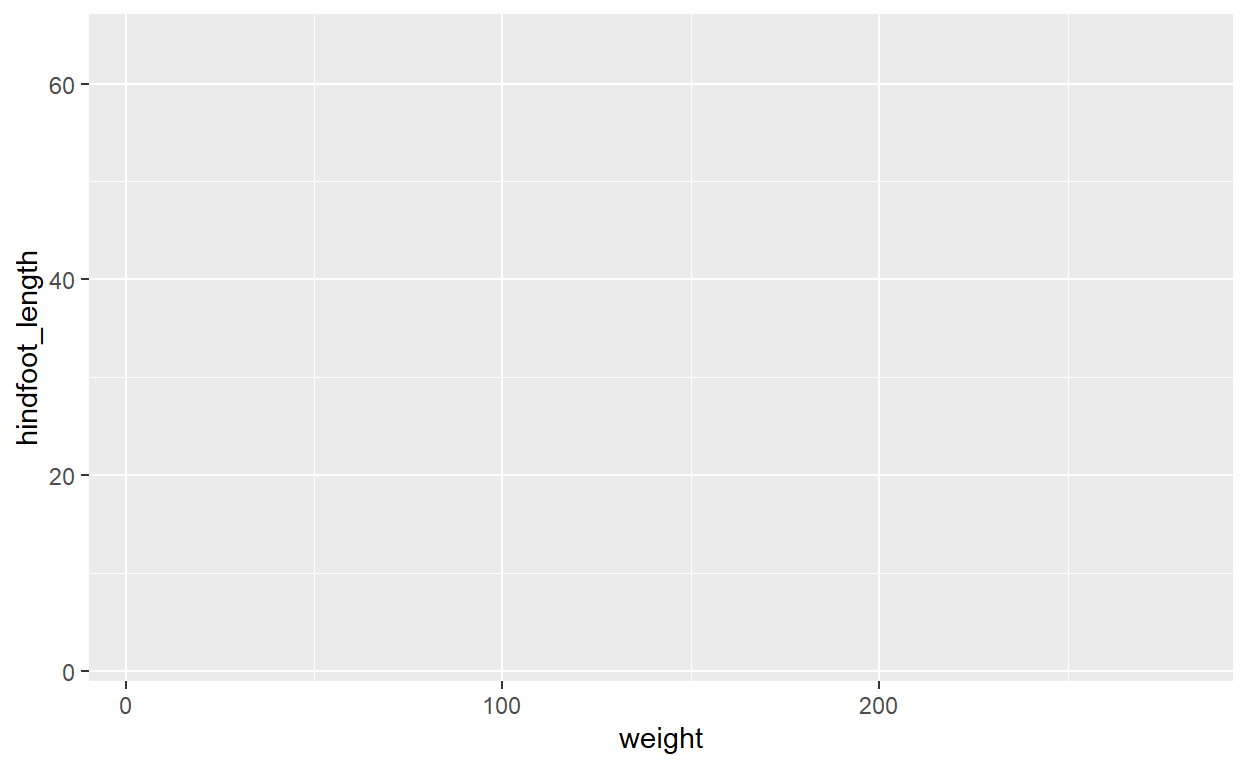
\includegraphics{data_visualization_ggplot_17Feb2021_files/figure-latex/define-mapping-1.pdf}

\begin{Shaded}
\begin{Highlighting}[]
\CommentTok{\#}
\CommentTok{\# Creates a blank ggplot(), with the variables mapped to the x{-} and y{-}axis}
\CommentTok{\# ggplot() knows where the variables live, since you have defined the data to use}
\end{Highlighting}
\end{Shaded}
\item
  Add ``geoms'' -- graphical representations of the data in the plot
  (points, lines, bars). \textbf{\texttt{ggplot2}} offers many different
  geoms; we will use some common ones today, including:

  \begin{itemize}
  \tightlist
  \item
    \texttt{geom\_point()} for scatter plots, dot plots, etc.
  \item
    \texttt{geom\_boxplot()} for boxplots\\
  \item
    \texttt{geom\_bar()} for bar charts
  \item
    \texttt{geom\_line()} for trend lines, time series, etc.
  \end{itemize}
\end{enumerate}

To add a geom to the plot use the \texttt{+} operator. Because we have
two continuous variables in the data, let's use \texttt{geom\_point()}
first:

\begin{Shaded}
\begin{Highlighting}[]
\FunctionTok{ggplot}\NormalTok{(}\AttributeTok{data =}\NormalTok{ surveys, }
       \AttributeTok{mapping =} \FunctionTok{aes}\NormalTok{(}\AttributeTok{x =}\NormalTok{ weight, }\AttributeTok{y =}\NormalTok{ hindfoot\_length)) }\SpecialCharTok{+}
  \FunctionTok{geom\_point}\NormalTok{()}
\end{Highlighting}
\end{Shaded}

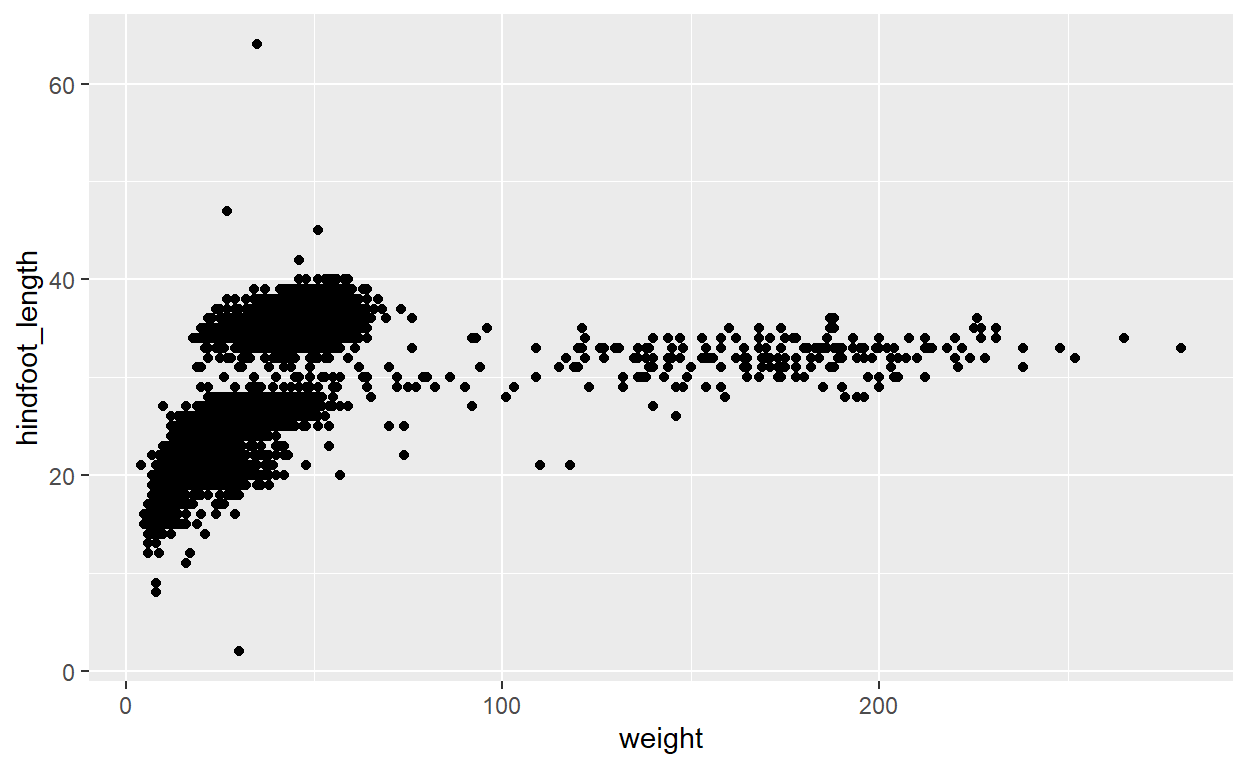
\includegraphics{data_visualization_ggplot_17Feb2021_files/figure-latex/add-to-plots-1.pdf}

\begin{Shaded}
\begin{Highlighting}[]
 \CommentTok{\# Adds a point for each row (observation) in the data  }
\end{Highlighting}
\end{Shaded}

You can think of the \texttt{+} sign as adding layers to the plot. Each
\texttt{+} sign must be placed at the end of the line containing the
\emph{previous} layer. If, instead, the \texttt{+} sign is added at the
beginning of the line containing the new layer,
\textbf{\texttt{ggplot2}} will not add the new layer and will return an
error message.

\begin{Shaded}
\begin{Highlighting}[]
\CommentTok{\# This will not add the new layer and will return an error message}
\FunctionTok{ggplot}\NormalTok{(}\AttributeTok{data =}\NormalTok{ surveys, }
       \AttributeTok{mapping =} \FunctionTok{aes}\NormalTok{(}\AttributeTok{x =}\NormalTok{ weight, }\AttributeTok{y =}\NormalTok{ hindfoot\_length)) }
  \SpecialCharTok{+} \FunctionTok{geom\_point}\NormalTok{()}
\end{Highlighting}
\end{Shaded}

\newpage

\hypertarget{building-plots-iteratively}{%
\subsubsection{Building Plots
Iteratively}\label{building-plots-iteratively}}

Building plots with \textbf{\texttt{ggplot2}} is typically an iterative
process. We start by defining the dataset we'll use, lay out the axes,
and choose a geom:

\begin{Shaded}
\begin{Highlighting}[]
\FunctionTok{ggplot}\NormalTok{(}\AttributeTok{data =}\NormalTok{ surveys, }
       \AttributeTok{mapping =} \FunctionTok{aes}\NormalTok{(}\AttributeTok{x =}\NormalTok{ weight, }\AttributeTok{y =}\NormalTok{ hindfoot\_length)) }\SpecialCharTok{+}
  \FunctionTok{geom\_point}\NormalTok{()}
\end{Highlighting}
\end{Shaded}

\includegraphics{data_visualization_ggplot_17Feb2021_files/figure-latex/build-plot-1.pdf}

Then, we start modifying this plot to extract more information from it.
For instance, we can add transparency (\texttt{alpha}) to the points, to
avoid overplotting:

\begin{Shaded}
\begin{Highlighting}[]
\FunctionTok{ggplot}\NormalTok{(}\AttributeTok{data =}\NormalTok{ surveys, }
       \AttributeTok{mapping =} \FunctionTok{aes}\NormalTok{(}\AttributeTok{x =}\NormalTok{ weight, }\AttributeTok{y =}\NormalTok{ hindfoot\_length)) }\SpecialCharTok{+}
  \FunctionTok{geom\_point}\NormalTok{(}\AttributeTok{alpha =} \FloatTok{0.1}\NormalTok{)}
\end{Highlighting}
\end{Shaded}

\includegraphics{data_visualization_ggplot_17Feb2021_files/figure-latex/modify-plot-1.pdf}

\begin{Shaded}
\begin{Highlighting}[]
\DocumentationTok{\#\# alpha reduces the opacity of the points }
\DocumentationTok{\#\# 0 is fully transparent}
\DocumentationTok{\#\# 1 is the original opacity}
\end{Highlighting}
\end{Shaded}

We can also add colors for all the points:

\begin{Shaded}
\begin{Highlighting}[]
\FunctionTok{ggplot}\NormalTok{(}\AttributeTok{data =}\NormalTok{ surveys, }
       \AttributeTok{mapping =} \FunctionTok{aes}\NormalTok{(}\AttributeTok{x =}\NormalTok{ weight, }\AttributeTok{y =}\NormalTok{ hindfoot\_length)) }\SpecialCharTok{+}
  \FunctionTok{geom\_point}\NormalTok{(}\AttributeTok{alpha =} \FloatTok{0.1}\NormalTok{, }\AttributeTok{color =} \StringTok{"blue"}\NormalTok{)}
\end{Highlighting}
\end{Shaded}

\includegraphics{data_visualization_ggplot_17Feb2021_files/figure-latex/color-plot-1.pdf}

\texttt{geom\_point} also accepts aesthetics of size and shape. The size
of a point is its width in mm. The shape of a point has five different
options for plotting:

\begin{itemize}
\tightlist
\item
  an integer {[}0, 25{]} of defined plotting characters -- same as base
  \texttt{R}
\item
  the name of the shape in quotations (e.g.~``circle open'' or ``diamond
  filled'')
\item
  a single character, to use that character as a plotting symbol
\item
  a ``.'' to draw the smallest point that is visible -- typically 1
  pixel
\item
  an NA, to draw nothing
\end{itemize}

Reference for shapes in integers and characters:\\
\url{https://ggplot2.tidyverse.org/articles/ggplot2-specs.html}

\begin{quote}
\mbox{}%
\hypertarget{challenge-1}{%
\paragraph{Challenge 1}\label{challenge-1}}

Copy and paste the code from the previous code chunk and modify it to
assign one of these aesthetics to the \texttt{geom\_point} aspect of
your plot.

What happened?
\end{quote}

\begin{Shaded}
\begin{Highlighting}[]
\DocumentationTok{\#\# Your ggplot code to answer the challenge goes here!}
\end{Highlighting}
\end{Shaded}

\newpage

\begin{Shaded}
\begin{Highlighting}[]
\FunctionTok{ggplot}\NormalTok{(}\AttributeTok{data =}\NormalTok{ surveys, }
       \AttributeTok{mapping =} \FunctionTok{aes}\NormalTok{(}\AttributeTok{x =}\NormalTok{ weight, }\AttributeTok{y =}\NormalTok{ hindfoot\_length)) }\SpecialCharTok{+}
  \FunctionTok{geom\_point}\NormalTok{(}\AttributeTok{alpha =} \FloatTok{0.1}\NormalTok{, }\AttributeTok{color =} \StringTok{"blue"}\NormalTok{, }\AttributeTok{shape =} \StringTok{"diamond"}\NormalTok{)}
\end{Highlighting}
\end{Shaded}

\includegraphics{data_visualization_ggplot_17Feb2021_files/figure-latex/challenge-1-solution-1.pdf}

\hypertarget{piping-data-in}{%
\subsubsection{Piping Data In}\label{piping-data-in}}

Because \textbf{\texttt{ggplot2}} lives in the \texttt{tidyverse}, it is
expected to work well with other packages in the \texttt{tidyverse}.
Because of this, the first argument to creating a \texttt{ggplot()} is
the dataset you wish to be working with. The pipe operator sends the
output of one function directly into the next function, which is useful
when you need to do many things to the same dataset. Since the dataset
we wish to use is the first argument to \texttt{ggplot()}, we can use
the pipe operator to pipe the data into the \texttt{ggplot()} function!

Pipes in \texttt{R} look like \texttt{\%\textgreater{}\%} and are made
available via the \textbf{\texttt{magrittr}} package, installed
automatically with the \textbf{\texttt{tidyverse}}. If you use RStudio,
you can type the pipe with Ctrl + Shift + M if you have a PC or Cmd +
Shift + M if you have a Mac.

This would instead look like this:

\begin{Shaded}
\begin{Highlighting}[]
\NormalTok{surveys }\SpecialCharTok{\%\textgreater{}\%}  
  \DocumentationTok{\#\# data to be used in the ggplot  }
  \FunctionTok{ggplot}\NormalTok{(}\AttributeTok{mapping =} \FunctionTok{aes}\NormalTok{(}\AttributeTok{x =}\NormalTok{ weight, }\AttributeTok{y =}\NormalTok{ hindfoot\_length)) }\SpecialCharTok{+} 
  \DocumentationTok{\#\# uses the data piped in as the first arguement to ggplot() }
  \FunctionTok{geom\_point}\NormalTok{(}\AttributeTok{alpha =} \FloatTok{0.1}\NormalTok{, }\AttributeTok{color =} \StringTok{"blue"}\NormalTok{)}
\end{Highlighting}
\end{Shaded}

\includegraphics{data_visualization_ggplot_17Feb2021_files/figure-latex/pipe-example-1.pdf}

Once we pipe the data in, the first argument becomes the
\texttt{mapping} of the aesthetics. Technically, we are using the name
of this argument, which is why it looks like:

\texttt{mapping\ =\ aes(\textless{}VARIABLES\textgreater{})}

When we pipe our data in, the first argument then becomes this
\texttt{mapping} argument.

\hypertarget{assigning-more-variables-to-aesthetics}{%
\subsubsection{Assigning More Variables to
Aesthetics}\label{assigning-more-variables-to-aesthetics}}

To color each species in the plot differently, you could use a vector as
an input to the argument \textbf{color}. \textbf{\texttt{ggplot2}} will
provide a different color corresponding to different values in the
vector. Here is an example where we color with
\textbf{\texttt{species\_id}}:

\begin{Shaded}
\begin{Highlighting}[]
\NormalTok{surveys }\SpecialCharTok{\%\textgreater{}\%} 
  \FunctionTok{ggplot}\NormalTok{(}\AttributeTok{mapping =} \FunctionTok{aes}\NormalTok{(}\AttributeTok{x =}\NormalTok{ weight, }\AttributeTok{y =}\NormalTok{ hindfoot\_length)) }\SpecialCharTok{+}
  \FunctionTok{geom\_point}\NormalTok{(}\AttributeTok{alpha =} \FloatTok{0.1}\NormalTok{, }\FunctionTok{aes}\NormalTok{(}\AttributeTok{color =}\NormalTok{ species\_id)) }
\end{Highlighting}
\end{Shaded}

\includegraphics{data_visualization_ggplot_17Feb2021_files/figure-latex/color-example1-1.pdf}

\textbf{Note:} When specifying an \texttt{alpha} for a scatterplot, it
automatically uses that \textbf{same} \texttt{alpha} in the legend. To
remedy this you can add:

\texttt{guides(color\ =\ guide\_legend(override.aes\ =\ list(alpha\ =\ 1)))}

to your plot. This customizes the legend appearance, similar to what we
will see in the customization section.

We can also specify the colors directly inside the mapping provided in
the \texttt{ggplot()} function. This will be seen by \textbf{any} geom
layers and the mapping will be determined by the x- and y-axis set up in
\texttt{aes()}.

\begin{Shaded}
\begin{Highlighting}[]
\NormalTok{surveys }\SpecialCharTok{\%\textgreater{}\%} 
  \FunctionTok{ggplot}\NormalTok{(}\AttributeTok{mapping =} \FunctionTok{aes}\NormalTok{(}\AttributeTok{x =}\NormalTok{ weight, }\AttributeTok{y =}\NormalTok{ hindfoot\_length, }\AttributeTok{color =}\NormalTok{ species\_id)) }\SpecialCharTok{+}
  \FunctionTok{geom\_point}\NormalTok{(}\AttributeTok{alpha =} \FloatTok{0.1}\NormalTok{)}
\end{Highlighting}
\end{Shaded}

\includegraphics{data_visualization_ggplot_17Feb2021_files/figure-latex/color-example2-1.pdf}

Notice that we can change the geom layer and colors will be still
determined by \textbf{\texttt{species\_id}}

\hypertarget{local-aesthetics-versus-global-aesthetics}{%
\subsubsection{Local Aesthetics versus Global
Aesthetics}\label{local-aesthetics-versus-global-aesthetics}}

When you define aesthetics in the \texttt{ggplot()} function, those
mappings hold for \textbf{every} aspect of your plot.

For example, if you chose to add a smoothing line to your plot of weight
versus hindfoot length, you would get different lines depending on where
you define your color aesthetics.

\textbf{Globally}

\begin{Shaded}
\begin{Highlighting}[]
\NormalTok{surveys }\SpecialCharTok{\%\textgreater{}\%} 
  \FunctionTok{ggplot}\NormalTok{(}\AttributeTok{mapping =} \FunctionTok{aes}\NormalTok{(}\AttributeTok{x =}\NormalTok{ weight, }\AttributeTok{y =}\NormalTok{ hindfoot\_length, }\AttributeTok{color =}\NormalTok{ species\_id)) }\SpecialCharTok{+}
  \FunctionTok{geom\_jitter}\NormalTok{(}\AttributeTok{alpha =} \FloatTok{0.1}\NormalTok{) }\SpecialCharTok{+} 
  \FunctionTok{geom\_smooth}\NormalTok{()}
\end{Highlighting}
\end{Shaded}

\begin{verbatim}
## `geom_smooth()` using method = 'gam' and formula 'y ~ s(x, bs = "cs")'
\end{verbatim}

\includegraphics{data_visualization_ggplot_17Feb2021_files/figure-latex/color-global-1.pdf}

\begin{Shaded}
\begin{Highlighting}[]
\DocumentationTok{\#\# smoothing line for each species\_id {-}{-} because color is defined globally}
\end{Highlighting}
\end{Shaded}

\textbf{Locally}

\begin{Shaded}
\begin{Highlighting}[]
\NormalTok{surveys }\SpecialCharTok{\%\textgreater{}\%} 
  \FunctionTok{ggplot}\NormalTok{(}\AttributeTok{mapping =} \FunctionTok{aes}\NormalTok{(}\AttributeTok{x =}\NormalTok{ weight, }\AttributeTok{y =}\NormalTok{ hindfoot\_length)) }\SpecialCharTok{+}
  \FunctionTok{geom\_jitter}\NormalTok{(}\FunctionTok{aes}\NormalTok{(}\AttributeTok{color =}\NormalTok{ species\_id), }\AttributeTok{alpha =} \FloatTok{0.1}\NormalTok{) }\SpecialCharTok{+} 
  \FunctionTok{geom\_smooth}\NormalTok{()}
\end{Highlighting}
\end{Shaded}

\begin{verbatim}
## `geom_smooth()` using method = 'gam' and formula 'y ~ s(x, bs = "cs")'
\end{verbatim}

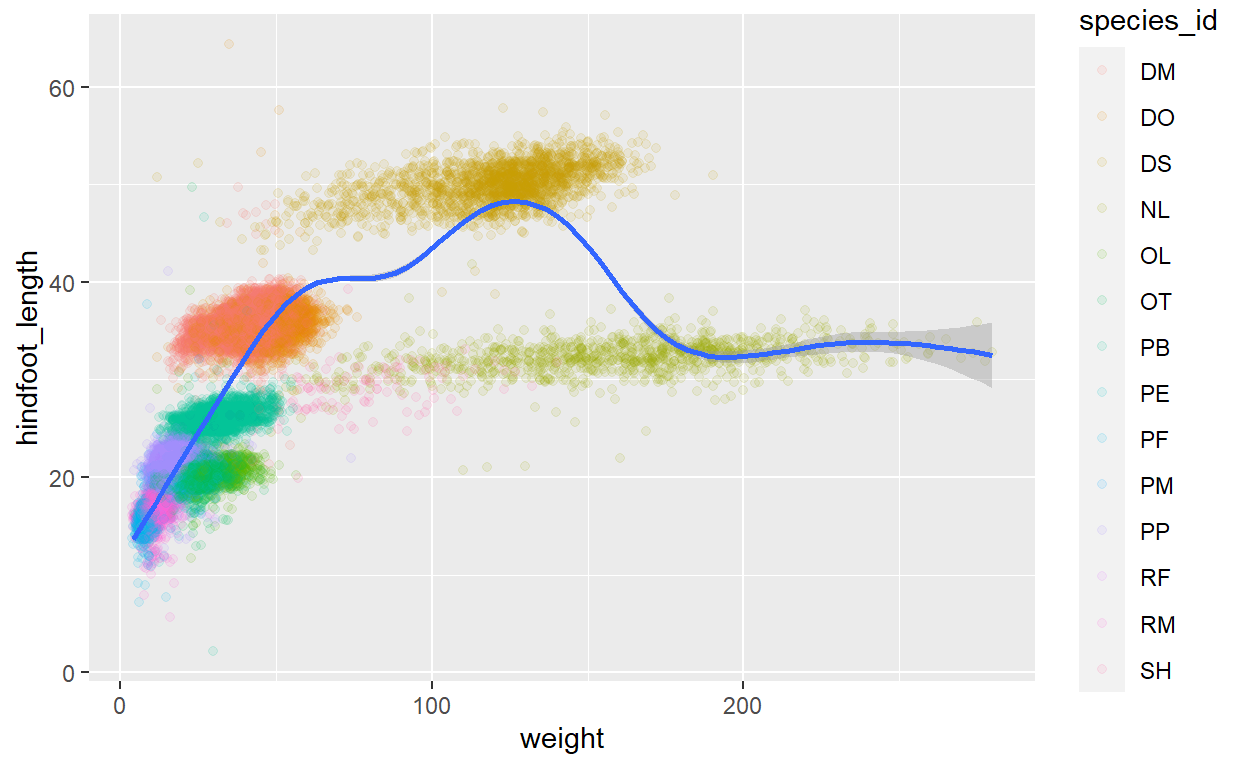
\includegraphics{data_visualization_ggplot_17Feb2021_files/figure-latex/unnamed-chunk-4-1.pdf}

\begin{Shaded}
\begin{Highlighting}[]
\DocumentationTok{\#\# one smoothing line {-}{-} no color defined globally}
\end{Highlighting}
\end{Shaded}

\begin{quote}
\mbox{}%
\hypertarget{challenge-2-part-1}{%
\paragraph{Challenge 2 (Part 1)}\label{challenge-2-part-1}}

Inspect the \texttt{geom\_point} help file (either go to
\url{https://ggplot2.tidyverse.org/reference/geom_point.html} or run
\texttt{?geom\_point}) to see what other aesthetics are available. Map a
new variable from the dataset to another aesthetic in your plot. What
happened? Does the aesthetic change if you use a continuous variable
versus a categorical/discrete variable?
\end{quote}

\begin{Shaded}
\begin{Highlighting}[]
\DocumentationTok{\#\# Your ggplot() code for the challenge goes here!}
\end{Highlighting}
\end{Shaded}

\begin{Shaded}
\begin{Highlighting}[]
\NormalTok{surveys }\SpecialCharTok{\%\textgreater{}\%} 
  \FunctionTok{ggplot}\NormalTok{(}\AttributeTok{mapping =} \FunctionTok{aes}\NormalTok{(}\AttributeTok{x =}\NormalTok{ weight, }\AttributeTok{y =}\NormalTok{ hindfoot\_length)) }\SpecialCharTok{+}
  \FunctionTok{geom\_jitter}\NormalTok{(}\FunctionTok{aes}\NormalTok{(}\AttributeTok{color =}\NormalTok{ plot\_type), }\AttributeTok{alpha =} \FloatTok{0.1}\NormalTok{) }\SpecialCharTok{+} 
  \FunctionTok{geom\_smooth}\NormalTok{()}
\end{Highlighting}
\end{Shaded}

\begin{verbatim}
## `geom_smooth()` using method = 'gam' and formula 'y ~ s(x, bs = "cs")'
\end{verbatim}

\includegraphics{data_visualization_ggplot_17Feb2021_files/figure-latex/challenge-2part1-solution-1.pdf}

\begin{quote}
\mbox{}%
\hypertarget{challenge-2-part-2}{%
\paragraph{Challenge 2 (Part 2)}\label{challenge-2-part-2}}

Use what you just learned to create a scatter plot of \texttt{weight}
over \texttt{plot\_id} with data from different plot types being showed
in different colors. Is this a good way to show this type of data?
\end{quote}

\begin{Shaded}
\begin{Highlighting}[]
\DocumentationTok{\#\# Your ggplot() code for the challenge goes here!}
\end{Highlighting}
\end{Shaded}

\begin{Shaded}
\begin{Highlighting}[]
\NormalTok{surveys }\SpecialCharTok{\%\textgreater{}\%} 
  \FunctionTok{ggplot}\NormalTok{(}\AttributeTok{mapping =} \FunctionTok{aes}\NormalTok{(}\AttributeTok{x =}\NormalTok{ plot\_id, }\AttributeTok{y =}\NormalTok{ weight)) }\SpecialCharTok{+}
  \FunctionTok{geom\_jitter}\NormalTok{(}\FunctionTok{aes}\NormalTok{(}\AttributeTok{color =}\NormalTok{ plot\_type), }\AttributeTok{alpha =} \FloatTok{0.1}\NormalTok{) }\SpecialCharTok{+} 
  \FunctionTok{geom\_smooth}\NormalTok{()}
\end{Highlighting}
\end{Shaded}

\begin{verbatim}
## `geom_smooth()` using method = 'gam' and formula 'y ~ s(x, bs = "cs")'
\end{verbatim}

\includegraphics{data_visualization_ggplot_17Feb2021_files/figure-latex/challenge-2part2-solution-1.pdf}

\hypertarget{boxplots-violin-plots}{%
\subsubsection{Boxplots \& Violin Plots}\label{boxplots-violin-plots}}

Boxplots provide a visualization of a quantitative variables across
different levels of a categorical (grouping) variable. For example, we
can use boxplots to visualize the distribution of weight within each
species:

\begin{Shaded}
\begin{Highlighting}[]
\NormalTok{surveys }\SpecialCharTok{\%\textgreater{}\%} 
  \FunctionTok{ggplot}\NormalTok{(}\AttributeTok{mapping =} \FunctionTok{aes}\NormalTok{(}\AttributeTok{x =}\NormalTok{ species\_id, }\AttributeTok{y =}\NormalTok{ weight)) }\SpecialCharTok{+}
  \FunctionTok{geom\_boxplot}\NormalTok{()}
\end{Highlighting}
\end{Shaded}

\includegraphics{data_visualization_ggplot_17Feb2021_files/figure-latex/boxplot1-1.pdf}

By adding points to boxplot, we can have a better idea of the number of
measurements and their distribution:

\begin{Shaded}
\begin{Highlighting}[]
\NormalTok{surveys }\SpecialCharTok{\%\textgreater{}\%} 
  \FunctionTok{ggplot}\NormalTok{(}\AttributeTok{mapping =} \FunctionTok{aes}\NormalTok{(}\AttributeTok{x =}\NormalTok{ species\_id, }\AttributeTok{y =}\NormalTok{ weight)) }\SpecialCharTok{+}
  \FunctionTok{geom\_boxplot}\NormalTok{(}\AttributeTok{alpha =} \DecValTok{0}\NormalTok{) }\SpecialCharTok{+} 
  \DocumentationTok{\#\# alpha = 0 eliminates the black (possible outlier) points, so they\textquotesingle{}re not plotted twice}
  \FunctionTok{geom\_jitter}\NormalTok{(}\AttributeTok{alpha =} \FloatTok{0.1}\NormalTok{, }\AttributeTok{color =} \StringTok{"tomato"}\NormalTok{)}
\end{Highlighting}
\end{Shaded}

\includegraphics{data_visualization_ggplot_17Feb2021_files/figure-latex/boxplot2-1.pdf}

\begin{Shaded}
\begin{Highlighting}[]
\DocumentationTok{\#\# alpha = 0.1 decreases the opacity of the points, to not be too busy}
\end{Highlighting}
\end{Shaded}

\begin{quote}
Notice how the boxplot layer is behind the jitter layer? What would you
change in the code to put the boxplot in front of the points?
\end{quote}

\begin{quote}
\mbox{}%
\hypertarget{challenge-3-part-1}{%
\paragraph{Challenge 3 (Part 1)}\label{challenge-3-part-1}}

Boxplots are useful summaries, but hide details of the \emph{shape} of
the distribution. For example, if the distribution is bimodal, we would
not see it in a boxplot. A superior density plot is the violin plot,
where the shape (of the density of points) is drawn.

Replace the box plot with a violin plot. For help see
\texttt{geom\_violin()}. Start with the boxplot we created:
\end{quote}

\begin{Shaded}
\begin{Highlighting}[]
\FunctionTok{ggplot}\NormalTok{(}\AttributeTok{data =}\NormalTok{ surveys, }\AttributeTok{mapping =} \FunctionTok{aes}\NormalTok{(}\AttributeTok{x =}\NormalTok{ species\_id, }\AttributeTok{y =}\NormalTok{ weight)) }\SpecialCharTok{+}
  \FunctionTok{geom\_boxplot}\NormalTok{(}\AttributeTok{alpha =} \DecValTok{0}\NormalTok{) }\SpecialCharTok{+}
  \FunctionTok{geom\_jitter}\NormalTok{(}\AttributeTok{alpha =} \FloatTok{0.1}\NormalTok{, }\AttributeTok{color =} \StringTok{"tomato"}\NormalTok{)}
\end{Highlighting}
\end{Shaded}

\includegraphics{data_visualization_ggplot_17Feb2021_files/figure-latex/challenge-3part1-example-1.pdf}

\begin{Shaded}
\begin{Highlighting}[]
\DocumentationTok{\#\#  Start with the boxplot we created}
\DocumentationTok{\#\#  1. Replace the boxplot with a violin plot. For help, see geom\_violin().}
\DocumentationTok{\#\#  You might need to decrease opacity even more to see the violins (try 0.03)}
\end{Highlighting}
\end{Shaded}

\begin{Shaded}
\begin{Highlighting}[]
\NormalTok{surveys }\SpecialCharTok{\%\textgreater{}\%} 
  \FunctionTok{ggplot}\NormalTok{(}\AttributeTok{mapping =} \FunctionTok{aes}\NormalTok{(}\AttributeTok{x =}\NormalTok{ species\_id, }\AttributeTok{y =}\NormalTok{ weight)) }\SpecialCharTok{+}
  \FunctionTok{geom\_violin}\NormalTok{() }\SpecialCharTok{+} 
  \FunctionTok{geom\_jitter}\NormalTok{(}\AttributeTok{alpha =} \FloatTok{0.03}\NormalTok{, }\AttributeTok{color =} \StringTok{"tomato"}\NormalTok{)  }
\end{Highlighting}
\end{Shaded}

\includegraphics{data_visualization_ggplot_17Feb2021_files/figure-latex/challenge-3part1-solution-1.pdf}

\begin{quote}
\mbox{}%
\hypertarget{challenge-3-part-2}{%
\paragraph{Challenge 3 (Part 2)}\label{challenge-3-part-2}}

So far, we've looked at the distribution of weight within species. Let's
try making a new plot to explore the distribution of another variable
within each species.

Create a boxplot for \texttt{hindfoot\_length}. This time overlay the
boxplot layer over a jitter layer that shows the actual measurements.
\end{quote}

\begin{Shaded}
\begin{Highlighting}[]
\DocumentationTok{\#\#  First: create boxplot for hindfoot\_length\textasciigrave{} overlaid on a jitter layer.}
\end{Highlighting}
\end{Shaded}

\begin{Shaded}
\begin{Highlighting}[]
\NormalTok{surveys }\SpecialCharTok{\%\textgreater{}\%} 
  \FunctionTok{ggplot}\NormalTok{(}\AttributeTok{mapping =} \FunctionTok{aes}\NormalTok{(}\AttributeTok{x =}\NormalTok{ species\_id, }\AttributeTok{y =}\NormalTok{ hindfoot\_length)) }\SpecialCharTok{+}
  \FunctionTok{geom\_jitter}\NormalTok{(}\AttributeTok{alpha =} \FloatTok{0.3}\NormalTok{, }\AttributeTok{color =} \StringTok{"tomato"}\NormalTok{) }\SpecialCharTok{+}
  \FunctionTok{geom\_boxplot}\NormalTok{(}\AttributeTok{alpha =} \DecValTok{0}\NormalTok{) }
\end{Highlighting}
\end{Shaded}

\includegraphics{data_visualization_ggplot_17Feb2021_files/figure-latex/challenge-3part2-solution-1.pdf}

\begin{quote}
\mbox{}%
\hypertarget{challenge-3-part-3}{%
\paragraph{Challenge 3 (Part 3)}\label{challenge-3-part-3}}

Now, add color to the data points on your boxplot according to the plot
from which the sample was taken (\texttt{plot\_id}).

\emph{Hint:} Check the class for \texttt{plot\_id}. If \texttt{plot\_id}
was a character instead, how would the graph be different?
\end{quote}

\begin{Shaded}
\begin{Highlighting}[]
\DocumentationTok{\#\# Next: add color to the data points on your boxplot according to the}
\DocumentationTok{\#\# plot from which the sample was taken (plot\_id).}

\DocumentationTok{\#\# Hint: Check the class for plot\_id\textasciigrave{}. If plot\_id was a character instead, }
\DocumentationTok{\#\# how would the graph be different? }
\end{Highlighting}
\end{Shaded}

\begin{Shaded}
\begin{Highlighting}[]
\NormalTok{surveys }\SpecialCharTok{\%\textgreater{}\%} 
  \FunctionTok{ggplot}\NormalTok{(}\AttributeTok{mapping =} \FunctionTok{aes}\NormalTok{(}\AttributeTok{x =}\NormalTok{ species\_id, }\AttributeTok{y =}\NormalTok{ hindfoot\_length)) }\SpecialCharTok{+}
  \FunctionTok{geom\_jitter}\NormalTok{(}\AttributeTok{alpha =} \FloatTok{0.3}\NormalTok{, }\AttributeTok{mapping =} \FunctionTok{aes}\NormalTok{(}\AttributeTok{color =}\NormalTok{ plot\_id)) }\SpecialCharTok{+}
  \FunctionTok{geom\_boxplot}\NormalTok{(}\AttributeTok{alpha =} \DecValTok{0}\NormalTok{) }
\end{Highlighting}
\end{Shaded}

\includegraphics{data_visualization_ggplot_17Feb2021_files/figure-latex/challenge-3part3-solution-1.pdf}

\begin{Shaded}
\begin{Highlighting}[]
\DocumentationTok{\#\# Checking the data type for plot\_id}
\FunctionTok{class}\NormalTok{(surveys}\SpecialCharTok{$}\NormalTok{plot\_id)}
\end{Highlighting}
\end{Shaded}

\begin{verbatim}
## [1] "numeric"
\end{verbatim}

\begin{Shaded}
\begin{Highlighting}[]
\DocumentationTok{\#\# Creating a new variable named plot\_id\_chr}
\DocumentationTok{\#\# which is the character version of plot\_id}
\NormalTok{surveys }\OtherTok{\textless{}{-}}\NormalTok{ surveys }\SpecialCharTok{\%\textgreater{}\%} 
  \FunctionTok{mutate}\NormalTok{(}\AttributeTok{plot\_id\_chr =} \FunctionTok{as.character}\NormalTok{(plot\_id))}

\DocumentationTok{\#\# Using new character plot\_id to make a boxplot}
\NormalTok{surveys }\SpecialCharTok{\%\textgreater{}\%} 
  \FunctionTok{ggplot}\NormalTok{(}\AttributeTok{mapping =} \FunctionTok{aes}\NormalTok{(}\AttributeTok{x =}\NormalTok{ species\_id, }\AttributeTok{y =}\NormalTok{ hindfoot\_length)) }\SpecialCharTok{+}
  \FunctionTok{geom\_jitter}\NormalTok{(}\AttributeTok{alpha =} \FloatTok{0.3}\NormalTok{, }\AttributeTok{mapping =} \FunctionTok{aes}\NormalTok{(}\AttributeTok{color =}\NormalTok{ plot\_id\_chr)) }\SpecialCharTok{+}  
  \FunctionTok{geom\_boxplot}\NormalTok{(}\AttributeTok{alpha =} \DecValTok{0}\NormalTok{)  }
\end{Highlighting}
\end{Shaded}

\includegraphics{data_visualization_ggplot_17Feb2021_files/figure-latex/challenge-3part3-solution-2.pdf}

\hypertarget{plotting-single-variables}{%
\subsection{Plotting Single Variables}\label{plotting-single-variables}}

\hypertarget{distribution-plots-quantitative-variables}{%
\subsubsection{Distribution Plots (Quantitative
Variables)}\label{distribution-plots-quantitative-variables}}

If we wish to visualize the distribution of a single quantitative
variable, our plot changes a bit. Unfortunately, the
\texttt{geom\_violin()} function only accepts groups, so we cannot make
a violin plot with no groups. Darn it!

But, a violin is simply a density plot that's been reflected across the
y-axis. So, we could likely suffice with a density plot.

To visualize the distribution of rodent weights we could aggregate over
all species, years, plots, etc. and produce a single density plot:

\begin{Shaded}
\begin{Highlighting}[]
\NormalTok{surveys }\SpecialCharTok{\%\textgreater{}\%} 
  \FunctionTok{ggplot}\NormalTok{(}\AttributeTok{mapping =} \FunctionTok{aes}\NormalTok{(}\AttributeTok{x =}\NormalTok{ weight)) }\SpecialCharTok{+} 
  \FunctionTok{geom\_density}\NormalTok{()}
\end{Highlighting}
\end{Shaded}

\includegraphics{data_visualization_ggplot_17Feb2021_files/figure-latex/dist-plot-1.pdf}

The default is an empty density plot, which is largely unsatisfying. By
adding a \texttt{fill\ =\ \textless{}COLOR\textgreater{}} argument to
\texttt{geom\_density()} we can produce a nicer looking plot:

\begin{Shaded}
\begin{Highlighting}[]
\NormalTok{surveys }\SpecialCharTok{\%\textgreater{}\%} 
  \FunctionTok{ggplot}\NormalTok{(}\AttributeTok{mapping =} \FunctionTok{aes}\NormalTok{(}\AttributeTok{x =}\NormalTok{ weight)) }\SpecialCharTok{+} 
  \FunctionTok{geom\_density}\NormalTok{(}\AttributeTok{fill =} \StringTok{"sky blue"}\NormalTok{)}
\end{Highlighting}
\end{Shaded}

\includegraphics{data_visualization_ggplot_17Feb2021_files/figure-latex/dist-add-color-1.pdf}

Another frequently used plot for a single quantitative variable is the
histogram. The same plot as above can be recreated using
\texttt{geom\_histogram()} instead of \texttt{geom\_density()}. However,
when you use \texttt{geom\_histogram()} it gives you a warning.

\begin{Shaded}
\begin{Highlighting}[]
\NormalTok{surveys }\SpecialCharTok{\%\textgreater{}\%} 
  \FunctionTok{ggplot}\NormalTok{(}\AttributeTok{mapping =} \FunctionTok{aes}\NormalTok{(}\AttributeTok{x =}\NormalTok{ weight)) }\SpecialCharTok{+} 
  \FunctionTok{geom\_histogram}\NormalTok{()}
\end{Highlighting}
\end{Shaded}

\begin{verbatim}
## `stat_bin()` using `bins = 30`. Pick better value with `binwidth`.
\end{verbatim}

\includegraphics{data_visualization_ggplot_17Feb2021_files/figure-latex/hist-1.pdf}

\begin{quote}
What warning do you get and why? Do you get an error like this when you
use \texttt{hist()} in base \texttt{R}?
\end{quote}

I was once told that the idea behind a good histogram was to make the
plot look as smooth as possible -- think about having it resemble the
continuous shape of the density plot.

\begin{quote}
\mbox{}%
\hypertarget{challenge-4}{%
\paragraph{Challenge 4}\label{challenge-4}}

Use the \texttt{bins} argument in \texttt{geom\_histogram()} to play
around with the number of bins in your histogram. Try different numbers
of bins to explore how that changes the results!
\end{quote}

\begin{Shaded}
\begin{Highlighting}[]
\DocumentationTok{\#\# Your code to answer the challenge goes here!}
\end{Highlighting}
\end{Shaded}

\begin{Shaded}
\begin{Highlighting}[]
\NormalTok{surveys }\SpecialCharTok{\%\textgreater{}\%} 
  \FunctionTok{ggplot}\NormalTok{(}\FunctionTok{aes}\NormalTok{(}\AttributeTok{x =}\NormalTok{ weight)) }\SpecialCharTok{+} 
  \FunctionTok{geom\_histogram}\NormalTok{(}\AttributeTok{fill =} \StringTok{"sky blue"}\NormalTok{ , }\AttributeTok{bins =} \DecValTok{50}\NormalTok{)}
\end{Highlighting}
\end{Shaded}

\includegraphics{data_visualization_ggplot_17Feb2021_files/figure-latex/challenge-4-solution-1.pdf}

\hypertarget{bar-charts-categorical-variables}{%
\subsubsection{Bar Charts (Categorical
Variables)}\label{bar-charts-categorical-variables}}

At first glimpse, you would think that a bar plot would be simple to
create, but bar plots reveal a subtle nuance of the plots we have
created thus far. The following bar chart displays the total number of
rodents in the \texttt{surveys} dataset, grouped by their species ID.

\begin{Shaded}
\begin{Highlighting}[]
\NormalTok{surveys }\SpecialCharTok{\%\textgreater{}\%} 
  \FunctionTok{ggplot}\NormalTok{(}\AttributeTok{mapping =} \FunctionTok{aes}\NormalTok{(}\AttributeTok{x =}\NormalTok{ species\_id)) }\SpecialCharTok{+} 
  \FunctionTok{geom\_bar}\NormalTok{()}
\end{Highlighting}
\end{Shaded}

\includegraphics{data_visualization_ggplot_17Feb2021_files/figure-latex/bar1-1.pdf}

The x-axis displays the levels of \texttt{species\_id}, a variable in
the \texttt{surveys} dataset. On the y-axis \texttt{count} is displayed,
but \texttt{count} is \textbf{not} a variable in our dataset! Where did
\texttt{count} come from? Graphs, such as the scatterplots, display the
raw values of your data. Other graphs, like bar charts and boxplots,
calculate new values (from your data) to plot.

\begin{itemize}
\item
  Bar charts and histograms bin your data and then plot the number of
  observations that fall in each bin.
\item
  Boxplots find summaries of your data (min, max, quartiles, median) and
  plot those summaries in a tidy box, with ``potential outliers'' (data
  over 1.5*IQR from Q1 or Q3) plotted as points.
\item
  Smoothers (as used in \texttt{geom\_smooth}) fit a model to your data
  (you can specify, but we used the \texttt{gam} (generalized additive
  model from the \texttt{mgcv} package) default) and then plot the
  predicted means from that model (with associated 95\% confidence
  intervals).
\end{itemize}

To calculate each of these summaries of the data, \texttt{R} uses a
different statistical transformation, or \emph{stat} for short. With a
bar chart this looks like the following process:

\begin{enumerate}
\def\labelenumi{\arabic{enumi}.}
\tightlist
\item
  \texttt{geom\_bar} first looks at the entire data frame\\
\item
  \texttt{geom\_bar} then transforms the data using the \texttt{count}
  statistic\\
\item
  the \texttt{count} statistic returns a data frame with the number of
  observations (rows) associated with each level of
  \texttt{species\_id}\\
\item
  \texttt{geom\_bar} uses this summary data frame, to build the plot --
  levels of \texttt{species\_id} are plotted on the x-axis and
  \texttt{count} is plotted on the y-axis
\end{enumerate}

Generally, you can use \texttt{geoms} and \texttt{stats}
interchangeably. This is because every \texttt{geom} has a default
\texttt{stat} and vice versa. For example, the following code produces
the same output as above:

\begin{Shaded}
\begin{Highlighting}[]
\NormalTok{surveys }\SpecialCharTok{\%\textgreater{}\%} 
  \FunctionTok{ggplot}\NormalTok{(}\AttributeTok{mapping =} \FunctionTok{aes}\NormalTok{(}\AttributeTok{x =}\NormalTok{ species\_id)) }\SpecialCharTok{+} 
  \FunctionTok{stat\_count}\NormalTok{()}
\end{Highlighting}
\end{Shaded}

\includegraphics{data_visualization_ggplot_17Feb2021_files/figure-latex/bar2-1.pdf}

If you so wish, you could override the default \texttt{stat} for that
\texttt{geom}. For example, if you wanted to plot a bar chart of
proportions you would use the following code to override the
\texttt{count} stat:

\begin{Shaded}
\begin{Highlighting}[]
\NormalTok{surveys }\SpecialCharTok{\%\textgreater{}\%} 
  \FunctionTok{ggplot}\NormalTok{(}\AttributeTok{mapping =} \FunctionTok{aes}\NormalTok{(}\AttributeTok{x =}\NormalTok{ species\_id)) }\SpecialCharTok{+} 
  \FunctionTok{geom\_bar}\NormalTok{(}\FunctionTok{aes}\NormalTok{(}\AttributeTok{y =} \FunctionTok{stat}\NormalTok{(prop), }\AttributeTok{group =} \DecValTok{1}\NormalTok{))}
\end{Highlighting}
\end{Shaded}

\includegraphics{data_visualization_ggplot_17Feb2021_files/figure-latex/bar3-1.pdf}

\begin{quote}
\mbox{}%
\hypertarget{challenge-5}{%
\paragraph{Challenge 5}\label{challenge-5}}

Why do we need to set \texttt{group\ =\ 1} in the above proportion bar
chart? In other words, what is wrong with the plot below?
\end{quote}

\begin{Shaded}
\begin{Highlighting}[]
\DocumentationTok{\#\# What is wrong with this plot? }
\NormalTok{surveys }\SpecialCharTok{\%\textgreater{}\%} 
  \FunctionTok{ggplot}\NormalTok{(}\AttributeTok{mapping =} \FunctionTok{aes}\NormalTok{(}\AttributeTok{x =}\NormalTok{ species\_id)) }\SpecialCharTok{+} 
  \FunctionTok{geom\_bar}\NormalTok{(}\FunctionTok{aes}\NormalTok{(}\AttributeTok{y =} \FunctionTok{stat}\NormalTok{(prop)))}
\end{Highlighting}
\end{Shaded}

\includegraphics{data_visualization_ggplot_17Feb2021_files/figure-latex/bar4-1.pdf}

\hypertarget{colored-andor-stacked-bar-charts}{%
\subsubsection{Colored and/or Stacked Bar
Charts}\label{colored-andor-stacked-bar-charts}}

Another piece of visual appeal to creating a bar chart is the ability to
use colors to differentiate the different groups, or to plot two
different variables in one bar chart (stacked bar chart). Let's start
with adding color to our bar chart.

\hypertarget{coloring-bars}{%
\paragraph{Coloring Bars}\label{coloring-bars}}

As we saw before, to add a color aesthetic to the plot we need to map it
to a variable. However, if we use the \texttt{color} option that we used
before we get a slightly unsatisfying result.

\begin{Shaded}
\begin{Highlighting}[]
\NormalTok{surveys }\SpecialCharTok{\%\textgreater{}\%} 
  \FunctionTok{ggplot}\NormalTok{(}\AttributeTok{mapping =} \FunctionTok{aes}\NormalTok{(}\AttributeTok{x =}\NormalTok{ species\_id, }\AttributeTok{color =}\NormalTok{ species\_id)) }\SpecialCharTok{+} 
  \FunctionTok{geom\_bar}\NormalTok{()}
\end{Highlighting}
\end{Shaded}

\includegraphics{data_visualization_ggplot_17Feb2021_files/figure-latex/bar5-1.pdf}

We notice that the color only appears in the outline of the bars. For a
bar chart, the aesthetic that we are interested in is the \texttt{fill}
of the bars.

\begin{quote}
\mbox{}%
\hypertarget{challenge-6}{%
\paragraph{Challenge 6}\label{challenge-6}}

Change the code below so that each bar is filled with a different color.
\end{quote}

\begin{Shaded}
\begin{Highlighting}[]
\NormalTok{surveys }\SpecialCharTok{\%\textgreater{}\%} 
  \FunctionTok{ggplot}\NormalTok{(}\AttributeTok{mapping =} \FunctionTok{aes}\NormalTok{(}\AttributeTok{x =}\NormalTok{ species\_id, }\AttributeTok{color =}\NormalTok{ species\_id)) }\SpecialCharTok{+} 
  \FunctionTok{geom\_bar}\NormalTok{()}
\end{Highlighting}
\end{Shaded}

\includegraphics{data_visualization_ggplot_17Feb2021_files/figure-latex/challenge-6-example-1.pdf}

\begin{Shaded}
\begin{Highlighting}[]
\NormalTok{surveys }\SpecialCharTok{\%\textgreater{}\%} 
  \FunctionTok{ggplot}\NormalTok{(}\AttributeTok{mapping =} \FunctionTok{aes}\NormalTok{(}\AttributeTok{x =}\NormalTok{ species\_id, }\AttributeTok{fill =}\NormalTok{ species\_id)) }\SpecialCharTok{+} 
  \FunctionTok{geom\_bar}\NormalTok{()}
\end{Highlighting}
\end{Shaded}

\includegraphics{data_visualization_ggplot_17Feb2021_files/figure-latex/challenge-6-solution-1.pdf}

\newpage

\hypertarget{stacking-bars}{%
\paragraph{Stacking Bars}\label{stacking-bars}}

Now suppose you are interested in whether the number of male and female
rodents captured differs by species. This would require for you to
create a bar plot with two categorical variables. You have two options:

\begin{enumerate}
\def\labelenumi{\arabic{enumi}.}
\tightlist
\item
  each of the bars for sex could be stacked within a species \emph{OR}
\item
  the bars for sex could be side-by-side within a species
\end{enumerate}

Let's see how the two approaches differ. To stack bars of a second
categorical variable we would instead use this second categorical
variable as the \texttt{fill} of the bars. Run these two lines of code
and see how they differ.

\begin{Shaded}
\begin{Highlighting}[]
\NormalTok{surveys }\SpecialCharTok{\%\textgreater{}\%} 
  \FunctionTok{ggplot}\NormalTok{(}\AttributeTok{mapping =} \FunctionTok{aes}\NormalTok{(}\AttributeTok{x =}\NormalTok{ species\_id, }\AttributeTok{fill =}\NormalTok{ sex)) }\SpecialCharTok{+} 
  \FunctionTok{geom\_bar}\NormalTok{()}
\end{Highlighting}
\end{Shaded}

\includegraphics{data_visualization_ggplot_17Feb2021_files/figure-latex/stacking-1.pdf}

\begin{Shaded}
\begin{Highlighting}[]
\NormalTok{surveys }\SpecialCharTok{\%\textgreater{}\%} 
  \FunctionTok{ggplot}\NormalTok{(}\AttributeTok{mapping =} \FunctionTok{aes}\NormalTok{(}\AttributeTok{x =}\NormalTok{ species\_id, }\AttributeTok{fill =}\NormalTok{ sex)) }\SpecialCharTok{+} 
  \FunctionTok{geom\_bar}\NormalTok{(}\AttributeTok{position =} \StringTok{"dodge"}\NormalTok{)}
\end{Highlighting}
\end{Shaded}

\includegraphics{data_visualization_ggplot_17Feb2021_files/figure-latex/stacking-2.pdf}

In the first plot, the position was chosen automatically, but in the
second plot the \texttt{position} argument was made explicit. What
changes did this make in the plots?

\hypertarget{time-series-data}{%
\subsection{Time-series Data}\label{time-series-data}}

Let's calculate number of counts per year for each genus.

\emph{What you will see in Data Wrangling:} First we need to group the
data and count records within each group!

\begin{Shaded}
\begin{Highlighting}[]
\NormalTok{yearly\_counts }\OtherTok{\textless{}{-}}\NormalTok{ surveys }\SpecialCharTok{\%\textgreater{}\%}
  \FunctionTok{count}\NormalTok{(year, genus) }
\DocumentationTok{\#\# counts the number of observations (rows) for each year, genus combination and creates a new variable "n"}
\end{Highlighting}
\end{Shaded}

Time series data can be visualized as a line plot with years on the
x-axis and counts on the y-axis:

\begin{Shaded}
\begin{Highlighting}[]
\NormalTok{yearly\_counts }\SpecialCharTok{\%\textgreater{}\%} 
  \FunctionTok{ggplot}\NormalTok{(}\AttributeTok{mapping =} \FunctionTok{aes}\NormalTok{(}\AttributeTok{x =}\NormalTok{ year, }\AttributeTok{y =}\NormalTok{ n)) }\SpecialCharTok{+}
  \FunctionTok{geom\_line}\NormalTok{()}
\end{Highlighting}
\end{Shaded}

\includegraphics{data_visualization_ggplot_17Feb2021_files/figure-latex/timeseries2-1.pdf}

Unfortunately, this does not work because we plotted data for all the
genera together. We need to tell \texttt{ggplot()} to draw a line for
each genus by modifying the aesthetic function to include
\texttt{group\ =\ genus}:

\begin{Shaded}
\begin{Highlighting}[]
\NormalTok{yearly\_counts }\SpecialCharTok{\%\textgreater{}\%} 
  \FunctionTok{ggplot}\NormalTok{(}\AttributeTok{mapping =} \FunctionTok{aes}\NormalTok{(}\AttributeTok{x =}\NormalTok{ year, }\AttributeTok{y =}\NormalTok{ n, }\AttributeTok{group =}\NormalTok{ genus)) }\SpecialCharTok{+}
  \FunctionTok{geom\_line}\NormalTok{()}
\end{Highlighting}
\end{Shaded}

\includegraphics{data_visualization_ggplot_17Feb2021_files/figure-latex/timeseries3-1.pdf}

Unfortunately, we can't tell what line corresponds to which genus. We
will be able to distinguish genera in the plot if we add colors (using
\texttt{color} also automatically groups the data):

\begin{Shaded}
\begin{Highlighting}[]
\NormalTok{yearly\_counts }\SpecialCharTok{\%\textgreater{}\%} 
\FunctionTok{ggplot}\NormalTok{(}\AttributeTok{mapping =} \FunctionTok{aes}\NormalTok{(}\AttributeTok{x =}\NormalTok{ year, }\AttributeTok{y =}\NormalTok{ n, }\AttributeTok{color =}\NormalTok{ genus)) }\SpecialCharTok{+}
    \FunctionTok{geom\_line}\NormalTok{()}
\end{Highlighting}
\end{Shaded}

\includegraphics{data_visualization_ggplot_17Feb2021_files/figure-latex/timeseries4-1.pdf}

\begin{quote}
\textbf{Note:} When specifying the color for a line graph, you don't
need to use both the
\texttt{color\ =\ \textless{}VARIABLE\textgreater{}} argument and the
\texttt{group\ =\ \textless{}VARIABLE\textgreater{}} argument. Both do
the same grouping of observations! So you just need to specify the
\texttt{color} argument.
\end{quote}

\hypertarget{faceting}{%
\subsubsection{Faceting}\label{faceting}}

\textbf{\texttt{ggplot2}} has a special technique called \emph{faceting}
that allows the user to split one plot into multiple plots based on a
categorical variable included in the dataset.

There are two types of \texttt{facet} functions:

\begin{itemize}
\tightlist
\item
  \texttt{facet\_wrap()} arranges a one-dimensional sequence of panels
  to allow them to cleanly fit on one page -- used for one variable
\item
  \texttt{facet\_grid()} allows you to form a matrix of rows and columns
  of panels -- used for two variables
\end{itemize}

Both geometries allow you to specify faceting variables specified within
the \texttt{vars()} function. The \texttt{vars()} function looks at the
categorical variable you provide it with and outputs the unique levels
(values) of that variable.

This looks like: \texttt{facet\_wrap(facets\ =\ vars(facet\_variable))}
or
\texttt{facet\_grid(rows\ =\ vars(row\_variable),\ cols\ =\ vars(col\_variable))}.

Let's start by using \texttt{facet\_wrap()} to make a time series plot
for each species:

\begin{Shaded}
\begin{Highlighting}[]
\NormalTok{yearly\_counts }\SpecialCharTok{\%\textgreater{}\%} 
  \FunctionTok{ggplot}\NormalTok{(}\AttributeTok{mapping =} \FunctionTok{aes}\NormalTok{(}\AttributeTok{x =}\NormalTok{ year, }\AttributeTok{y =}\NormalTok{ n)) }\SpecialCharTok{+}
  \FunctionTok{geom\_line}\NormalTok{() }\SpecialCharTok{+}
  \FunctionTok{facet\_wrap}\NormalTok{(}\AttributeTok{facets =} \FunctionTok{vars}\NormalTok{(genus))}
\end{Highlighting}
\end{Shaded}

\includegraphics{data_visualization_ggplot_17Feb2021_files/figure-latex/facet1-1.pdf}

Now we would like to split the line in each plot by the sex of the
rodent captured. To do that we need to make counts in the data frame
grouped by \texttt{year}, \texttt{species\_id}, and \texttt{sex}:

\begin{Shaded}
\begin{Highlighting}[]
\NormalTok{yearly\_sex\_counts }\OtherTok{\textless{}{-}}\NormalTok{ surveys }\SpecialCharTok{\%\textgreater{}\%}
  \FunctionTok{count}\NormalTok{(year, species\_id, sex)}
\DocumentationTok{\#\# counts the number of observations (rows) for each year, species, sex combination}
\end{Highlighting}
\end{Shaded}

We can now make the faceted plot by splitting further by sex using
\texttt{color} (within each panel):

\begin{Shaded}
\begin{Highlighting}[]
\NormalTok{yearly\_sex\_counts }\SpecialCharTok{\%\textgreater{}\%} 
  \FunctionTok{ggplot}\NormalTok{(}\AttributeTok{mapping =} \FunctionTok{aes}\NormalTok{(}\AttributeTok{x =}\NormalTok{ year, }\AttributeTok{y =}\NormalTok{ n, }\AttributeTok{color =}\NormalTok{ sex)) }\SpecialCharTok{+}
  \FunctionTok{geom\_line}\NormalTok{() }\SpecialCharTok{+}
  \FunctionTok{facet\_wrap}\NormalTok{(}\AttributeTok{facets =}  \FunctionTok{vars}\NormalTok{(species\_id))}
\end{Highlighting}
\end{Shaded}

\includegraphics{data_visualization_ggplot_17Feb2021_files/figure-latex/facet3-1.pdf}

You can also organize the panels only by rows (or only by columns),
using the optional \texttt{nrow} and \texttt{ncol} arguments:

\begin{Shaded}
\begin{Highlighting}[]
\NormalTok{yearly\_sex\_counts }\SpecialCharTok{\%\textgreater{}\%} 
  \FunctionTok{ggplot}\NormalTok{(}\AttributeTok{mapping =} \FunctionTok{aes}\NormalTok{(}\AttributeTok{x =}\NormalTok{ year, }\AttributeTok{y =}\NormalTok{ n, }\AttributeTok{color =}\NormalTok{ sex)) }\SpecialCharTok{+}
  \FunctionTok{geom\_line}\NormalTok{() }\SpecialCharTok{+}
  \FunctionTok{facet\_wrap}\NormalTok{(}\FunctionTok{vars}\NormalTok{(species\_id), }\AttributeTok{ncol =} \DecValTok{1}\NormalTok{)}
\end{Highlighting}
\end{Shaded}

\includegraphics{data_visualization_ggplot_17Feb2021_files/figure-latex/facet4-1.pdf}

\begin{Shaded}
\begin{Highlighting}[]
\CommentTok{\# One column, facet by rows}
\end{Highlighting}
\end{Shaded}

\begin{Shaded}
\begin{Highlighting}[]
\NormalTok{yearly\_sex\_counts }\SpecialCharTok{\%\textgreater{}\%} 
  \FunctionTok{ggplot}\NormalTok{(}\AttributeTok{mapping =} \FunctionTok{aes}\NormalTok{(}\AttributeTok{x =}\NormalTok{ year, }\AttributeTok{y =}\NormalTok{ n, }\AttributeTok{color =}\NormalTok{ sex)) }\SpecialCharTok{+}
  \FunctionTok{geom\_line}\NormalTok{() }\SpecialCharTok{+}
  \FunctionTok{facet\_wrap}\NormalTok{(}\FunctionTok{vars}\NormalTok{(species\_id), }\AttributeTok{nrow =} \DecValTok{1}\NormalTok{)}
\end{Highlighting}
\end{Shaded}

\includegraphics{data_visualization_ggplot_17Feb2021_files/figure-latex/facet5-1.pdf}

\begin{Shaded}
\begin{Highlighting}[]
\CommentTok{\# One row, facet by columns}
\end{Highlighting}
\end{Shaded}

Now let's use \texttt{facet\_grid()} to control how panels are organised
by both rows and columns:

\begin{Shaded}
\begin{Highlighting}[]
\NormalTok{yearly\_sex\_counts }\SpecialCharTok{\%\textgreater{}\%} 
  \FunctionTok{ggplot}\NormalTok{(}\AttributeTok{mapping =} \FunctionTok{aes}\NormalTok{(}\AttributeTok{x =}\NormalTok{ year, }\AttributeTok{y =}\NormalTok{ n, }\AttributeTok{color =}\NormalTok{ sex)) }\SpecialCharTok{+}
    \FunctionTok{geom\_line}\NormalTok{() }\SpecialCharTok{+}
    \FunctionTok{facet\_grid}\NormalTok{(}\AttributeTok{rows =} \FunctionTok{vars}\NormalTok{(sex), }\AttributeTok{cols =}  \FunctionTok{vars}\NormalTok{(species\_id))}
\end{Highlighting}
\end{Shaded}

\includegraphics{data_visualization_ggplot_17Feb2021_files/figure-latex/facet6-1.pdf}

\begin{quote}
\mbox{}%
\hypertarget{challenge-7}{%
\paragraph{Challenge 7}\label{challenge-7}}

Use what you just learned to create a plot that depicts how the average
weight of each species changes through the years. Play around with which
variable you facet by versus plot by!
\end{quote}

\begin{Shaded}
\begin{Highlighting}[]
\DocumentationTok{\#\# To get you started:  }
\NormalTok{yearly\_species\_weight }\OtherTok{\textless{}{-}}\NormalTok{ surveys }\SpecialCharTok{\%\textgreater{}\%} 
  \FunctionTok{group\_by}\NormalTok{(year, species\_id) }\SpecialCharTok{\%\textgreater{}\%}
  \DocumentationTok{\#\# Variables to group by}
  \FunctionTok{summarize}\NormalTok{(}\AttributeTok{avg\_weight =} \FunctionTok{mean}\NormalTok{(weight))}

\NormalTok{yearly\_species\_weight }\SpecialCharTok{\%\textgreater{}\%}
  \FunctionTok{ggplot}\NormalTok{(}\AttributeTok{mapping =} \FunctionTok{aes}\NormalTok{(}\AttributeTok{x =}\NormalTok{ year, }\AttributeTok{y =}\NormalTok{ n, }\AttributeTok{color =}\NormalTok{ avg\_weight)) }\SpecialCharTok{+}
    \FunctionTok{geom\_line}\NormalTok{() }\SpecialCharTok{+}
    \FunctionTok{facet\_wrap}\NormalTok{(}\AttributeTok{facets =}  \FunctionTok{vars}\NormalTok{(species\_id))}
\DocumentationTok{\#\# Your ggplot() code for the plot goes here!}
\end{Highlighting}
\end{Shaded}

\begin{Shaded}
\begin{Highlighting}[]
\DocumentationTok{\#\# To get you started:  }
\NormalTok{yearly\_species\_weight }\OtherTok{\textless{}{-}}\NormalTok{ surveys }\SpecialCharTok{\%\textgreater{}\%} 
  \DocumentationTok{\#\# Variables to group by:}
  \FunctionTok{group\_by}\NormalTok{(year, species\_id) }\SpecialCharTok{\%\textgreater{}\%}
  \FunctionTok{summarize}\NormalTok{(}\AttributeTok{avg\_weight =} \FunctionTok{mean}\NormalTok{(weight))}
\end{Highlighting}
\end{Shaded}

\begin{verbatim}
## `summarise()` regrouping output by 'year' (override with `.groups` argument)
\end{verbatim}

\begin{Shaded}
\begin{Highlighting}[]
\DocumentationTok{\#\# Coloring by species id}
\NormalTok{yearly\_species\_weight }\SpecialCharTok{\%\textgreater{}\%} 
\FunctionTok{ggplot}\NormalTok{(}\AttributeTok{mapping =} \FunctionTok{aes}\NormalTok{(}\AttributeTok{x =}\NormalTok{ year, }\AttributeTok{y =}\NormalTok{ avg\_weight, }\AttributeTok{color =}\NormalTok{ species\_id)) }\SpecialCharTok{+}
    \FunctionTok{geom\_line}\NormalTok{()}
\end{Highlighting}
\end{Shaded}

\includegraphics{data_visualization_ggplot_17Feb2021_files/figure-latex/challenge-7-solution-1.pdf}

\begin{Shaded}
\begin{Highlighting}[]
\DocumentationTok{\#\# Faceting by species id}
\NormalTok{yearly\_species\_weight }\SpecialCharTok{\%\textgreater{}\%} 
\FunctionTok{ggplot}\NormalTok{(}\AttributeTok{mapping =} \FunctionTok{aes}\NormalTok{(}\AttributeTok{x =}\NormalTok{ year, }\AttributeTok{y =}\NormalTok{ avg\_weight, }\AttributeTok{color =}\NormalTok{ species\_id)) }\SpecialCharTok{+}
    \FunctionTok{geom\_line}\NormalTok{() }\SpecialCharTok{+} 
  \FunctionTok{facet\_wrap}\NormalTok{(}\FunctionTok{vars}\NormalTok{(species\_id))}
\end{Highlighting}
\end{Shaded}

\includegraphics{data_visualization_ggplot_17Feb2021_files/figure-latex/challenge-7-solution-2.pdf}

\hypertarget{ggplot2-themes}{%
\subsection{\texorpdfstring{\textbf{\texttt{ggplot2}}
Themes}{ggplot2 Themes}}\label{ggplot2-themes}}

Usually plots with white background look more readable when printed.
Every single component of a \texttt{ggplot()} graph can be customized
using the generic \texttt{theme()} function, as we will see below.
However, there are pre-loaded themes available that change the overall
appearance of the graph without much effort.

For example, we can change our previous graph to have a simpler white
background using the \texttt{theme\_bw()} function:

\begin{Shaded}
\begin{Highlighting}[]
\NormalTok{yearly\_sex\_counts }\SpecialCharTok{\%\textgreater{}\%} 
 \FunctionTok{ggplot}\NormalTok{(}\AttributeTok{mapping =} \FunctionTok{aes}\NormalTok{(}\AttributeTok{x =}\NormalTok{ year, }\AttributeTok{y =}\NormalTok{ n, }\AttributeTok{color =}\NormalTok{ sex)) }\SpecialCharTok{+}
     \FunctionTok{geom\_line}\NormalTok{() }\SpecialCharTok{+}
     \FunctionTok{facet\_wrap}\NormalTok{(}\FunctionTok{vars}\NormalTok{(species\_id)) }\SpecialCharTok{+}
     \FunctionTok{theme\_bw}\NormalTok{()}
\end{Highlighting}
\end{Shaded}

\includegraphics{data_visualization_ggplot_17Feb2021_files/figure-latex/themes1-1.pdf}

In addition to \texttt{theme\_bw()}, which changes the plot background
to white, \textbf{\texttt{ggplot2}}comes with several other themes which
can be useful to quickly change the look of your visualization. The
complete list of themes is available at
\url{https://ggplot2.tidyverse.org/reference/ggtheme.html}.
\texttt{theme\_minimal()} and \texttt{theme\_light()} are popular, and
\texttt{theme\_void()} can be useful as a starting point to create a new
hand-crafted theme.

The
\href{https://jrnold.github.io/ggthemes/reference/index.html}{ggthemes}
package provides a wide variety of options. The
\href{https://exts.ggplot2.tidyverse.org/}{\textbf{\texttt{ggplot2}}
extensions website} provides a list of packages that extend the
capabilities of \textbf{\texttt{ggplot2}}, including additional themes.

\begin{quote}
\mbox{}%
\hypertarget{challenge-8}{%
\paragraph{Challenge 8}\label{challenge-8}}

Use what you just learned to add the plotting background theme of your
choosing to the plot you made in Challenge 7!
\end{quote}

\begin{Shaded}
\begin{Highlighting}[]
\DocumentationTok{\#\# Your ggplot() code for the plot goes here!}
\end{Highlighting}
\end{Shaded}

\begin{Shaded}
\begin{Highlighting}[]
\NormalTok{yearly\_species\_weight }\SpecialCharTok{\%\textgreater{}\%} 
  \FunctionTok{ggplot}\NormalTok{(}\AttributeTok{mapping =} \FunctionTok{aes}\NormalTok{(}\AttributeTok{x =}\NormalTok{ year, }\AttributeTok{y =}\NormalTok{ avg\_weight, }\AttributeTok{color =}\NormalTok{ species\_id)) }\SpecialCharTok{+}
  \FunctionTok{geom\_line}\NormalTok{() }\SpecialCharTok{+} 
  \FunctionTok{theme\_classic}\NormalTok{()}
\end{Highlighting}
\end{Shaded}

\includegraphics{data_visualization_ggplot_17Feb2021_files/figure-latex/challenge-8-solution-1.pdf}

\hypertarget{customization}{%
\subsection{Customization}\label{customization}}

Take a look at the
\href{https://github.com/rstudio/cheatsheets/raw/master/data-visualization-2.1.pdf}{\textbf{\texttt{ggplot2}}
cheat sheet}, and think of ways you could improve the previous plot.

\hypertarget{plot-labels}{%
\subsubsection{Plot Labels}\label{plot-labels}}

Now, let's change names of axes to something more informative than
`year' and `n' and add a title to the figure. Label customizations are
done using the \texttt{labs()} function like so:

\begin{Shaded}
\begin{Highlighting}[]
\NormalTok{yearly\_sex\_counts }\SpecialCharTok{\%\textgreater{}\%} 
  \FunctionTok{ggplot}\NormalTok{(}\AttributeTok{mapping =} \FunctionTok{aes}\NormalTok{(}\AttributeTok{x =}\NormalTok{ year, }\AttributeTok{y =}\NormalTok{ n, }\AttributeTok{color =}\NormalTok{ sex)) }\SpecialCharTok{+}
  \FunctionTok{geom\_line}\NormalTok{() }\SpecialCharTok{+}
  \FunctionTok{facet\_wrap}\NormalTok{(}\FunctionTok{vars}\NormalTok{(species\_id)) }\SpecialCharTok{+}
  \FunctionTok{theme\_bw}\NormalTok{() }\SpecialCharTok{+}
  \FunctionTok{labs}\NormalTok{(}\AttributeTok{title =} \StringTok{"Observed Genera Through Time"}\NormalTok{,}
       \AttributeTok{x =} \StringTok{"Year of Observation"}\NormalTok{,}
       \AttributeTok{y =} \StringTok{"Number of Rodents"}\NormalTok{,  }
       \AttributeTok{color =} \StringTok{"Sex"}\NormalTok{) }
\end{Highlighting}
\end{Shaded}

\includegraphics{data_visualization_ggplot_17Feb2021_files/figure-latex/labels-1.pdf}

\begin{quote}
\textbf{Tip: Wrapping Titles}

Sometimes the titles we wish to have for our plots are longer than the
space originally allotted. If you create a title and the text is running
off the plot you can add a \texttt{\textbackslash{}n} inside your title
to force a line break (\texttt{\textbackslash{}n} stands for new line).
\end{quote}

\hypertarget{label-plot-fonts}{%
\subsubsection{Label \& Plot Fonts}\label{label-plot-fonts}}

Note that it is also possible to change the fonts of your plots. If you
are on Windows, you may have to install the
\href{https://github.com/wch/extrafont}{\textbf{\texttt{extrafont}}
package}, and follow the instructions included in the README for this
package.

In the last plot, the axes have more informative names, but their
readability can be improved by increasing the font size. This can be
done with the generic \texttt{theme()} function.

\begin{Shaded}
\begin{Highlighting}[]
\NormalTok{yearly\_sex\_counts }\SpecialCharTok{\%\textgreater{}\%} 
  \FunctionTok{ggplot}\NormalTok{(}\AttributeTok{mapping =} \FunctionTok{aes}\NormalTok{(}\AttributeTok{x =}\NormalTok{ year, }\AttributeTok{y =}\NormalTok{ n, }\AttributeTok{color =}\NormalTok{ sex)) }\SpecialCharTok{+}
  \FunctionTok{geom\_line}\NormalTok{() }\SpecialCharTok{+}
  \FunctionTok{facet\_wrap}\NormalTok{(}\FunctionTok{vars}\NormalTok{(species\_id)) }\SpecialCharTok{+}
  \FunctionTok{theme\_bw}\NormalTok{() }\SpecialCharTok{+}
  \FunctionTok{labs}\NormalTok{(}\AttributeTok{title =} \StringTok{"Observed Genera Through Time"}\NormalTok{,}
       \AttributeTok{x =} \StringTok{"Year of Observation"}\NormalTok{,}
       \AttributeTok{y =} \StringTok{"Number of Rodents"}\NormalTok{, }
       \AttributeTok{color =} \StringTok{"Sex"}\NormalTok{) }\SpecialCharTok{+}
  \FunctionTok{theme}\NormalTok{(}\AttributeTok{text =} \FunctionTok{element\_text}\NormalTok{(}\AttributeTok{size =} \DecValTok{16}\NormalTok{))}
\end{Highlighting}
\end{Shaded}

\includegraphics{data_visualization_ggplot_17Feb2021_files/figure-latex/fonts-1.pdf}

\begin{Shaded}
\begin{Highlighting}[]
\DocumentationTok{\#\# sets ALL the text on the plot to be size 16}
\end{Highlighting}
\end{Shaded}

\textbf{Note:} \texttt{theme\_bw()} is a function for a
\textbf{specific} theme and \texttt{theme()} is a generic function for a
\textbf{variety} of different themes!

After our manipulations, you may notice that the values on the x-axis
are still not properly readable. Let's swap the orientation of the
labels, so the reader doesn't have to tilt their head when reading our
plot! The \texttt{coord\_flip()} function easily changes the x- and
y-axis.

\begin{Shaded}
\begin{Highlighting}[]
\NormalTok{yearly\_sex\_counts }\SpecialCharTok{\%\textgreater{}\%} 
  \FunctionTok{ggplot}\NormalTok{(}\AttributeTok{mapping =} \FunctionTok{aes}\NormalTok{(}\AttributeTok{x =}\NormalTok{ year, }\AttributeTok{y =}\NormalTok{ n, }\AttributeTok{color =}\NormalTok{ sex)) }\SpecialCharTok{+}
  \FunctionTok{geom\_line}\NormalTok{() }\SpecialCharTok{+}
  \FunctionTok{facet\_wrap}\NormalTok{(}\FunctionTok{vars}\NormalTok{(species\_id)) }\SpecialCharTok{+}
  \FunctionTok{theme\_bw}\NormalTok{() }\SpecialCharTok{+}
  \FunctionTok{labs}\NormalTok{(}\AttributeTok{title =} \StringTok{"Observed Genera by }\SpecialCharTok{\textbackslash{}n}\StringTok{ Year of Observation"}\NormalTok{,}
       \AttributeTok{x =} \StringTok{""}\NormalTok{,}
       \AttributeTok{y =} \StringTok{"Number of Rodents"}\NormalTok{, }
       \AttributeTok{color =} \StringTok{"Sex"}\NormalTok{) }\SpecialCharTok{+}
  \FunctionTok{theme}\NormalTok{(}\AttributeTok{text =} \FunctionTok{element\_text}\NormalTok{(}\AttributeTok{size =} \DecValTok{16}\NormalTok{)) }\SpecialCharTok{+} 
  \FunctionTok{coord\_flip}\NormalTok{()}
\end{Highlighting}
\end{Shaded}

\includegraphics{data_visualization_ggplot_17Feb2021_files/figure-latex/flip-1.pdf}

This definitely makes the reader tilt their head less! But, the text on
the x-axis is a bit too large to separate the numbers. We can specify
the text size for each element of the plot independently, if we so wish.
This would look something like this:

\begin{Shaded}
\begin{Highlighting}[]
\NormalTok{yearly\_sex\_counts }\SpecialCharTok{\%\textgreater{}\%} 
  \FunctionTok{ggplot}\NormalTok{(}\AttributeTok{mapping =} \FunctionTok{aes}\NormalTok{(}\AttributeTok{x =}\NormalTok{ year, }\AttributeTok{y =}\NormalTok{ n, }\AttributeTok{color =}\NormalTok{ sex)) }\SpecialCharTok{+}
  \FunctionTok{geom\_line}\NormalTok{() }\SpecialCharTok{+}
  \FunctionTok{facet\_wrap}\NormalTok{(}\FunctionTok{vars}\NormalTok{(species\_id)) }\SpecialCharTok{+}
  \FunctionTok{theme\_bw}\NormalTok{() }\SpecialCharTok{+}
  \FunctionTok{labs}\NormalTok{(}\AttributeTok{title =} \StringTok{"Observed Genera by Year of Observation"}\NormalTok{,}
       \AttributeTok{x =} \StringTok{""}\NormalTok{,}
       \AttributeTok{y =} \StringTok{"Number of Rodents"}\NormalTok{, }
       \AttributeTok{color =} \StringTok{"Sex"}\NormalTok{) }\SpecialCharTok{+}
  \FunctionTok{theme}\NormalTok{(}\AttributeTok{axis.text.x =} \FunctionTok{element\_text}\NormalTok{(}\AttributeTok{size =} \DecValTok{10}\NormalTok{), }
        \AttributeTok{axis.text.y =} \FunctionTok{element\_text}\NormalTok{(}\AttributeTok{size =} \DecValTok{12}\NormalTok{), }
        \AttributeTok{axis.title.x =} \FunctionTok{element\_text}\NormalTok{(}\AttributeTok{size =} \DecValTok{14}\NormalTok{),}
        \AttributeTok{legend.text =} \FunctionTok{element\_text}\NormalTok{(}\AttributeTok{size =} \DecValTok{12}\NormalTok{),}
        \AttributeTok{legend.title =} \FunctionTok{element\_text}\NormalTok{(}\AttributeTok{size =} \DecValTok{12}\NormalTok{),}
        \AttributeTok{plot.title =} \FunctionTok{element\_text}\NormalTok{(}\AttributeTok{size =} \DecValTok{16}\NormalTok{)) }\SpecialCharTok{+} 
  \FunctionTok{coord\_flip}\NormalTok{()}
\end{Highlighting}
\end{Shaded}

\includegraphics{data_visualization_ggplot_17Feb2021_files/figure-latex/text-size-1.pdf}

\hypertarget{legend-position}{%
\subsubsection{Legend Position}\label{legend-position}}

By default in \texttt{ggplot2} the legend is positioned on the right
hand side. However, you are able to change the position of the legend to
the left hand side, the top of the plot, or the bottom of the plot.

This is done by adding a \texttt{legend.position} theme to the plot's
\texttt{theme()}'s.

\begin{Shaded}
\begin{Highlighting}[]
\NormalTok{yearly\_sex\_counts }\SpecialCharTok{\%\textgreater{}\%} 
  \FunctionTok{ggplot}\NormalTok{(}\AttributeTok{mapping =} \FunctionTok{aes}\NormalTok{(}\AttributeTok{x =}\NormalTok{ year, }\AttributeTok{y =}\NormalTok{ n, }\AttributeTok{color =}\NormalTok{ sex)) }\SpecialCharTok{+}
  \FunctionTok{geom\_line}\NormalTok{() }\SpecialCharTok{+}
  \FunctionTok{facet\_wrap}\NormalTok{(}\FunctionTok{vars}\NormalTok{(species\_id)) }\SpecialCharTok{+}
  \FunctionTok{labs}\NormalTok{(}\AttributeTok{title =} \StringTok{"Observed Genera by Year of Observation by"}\NormalTok{,}
       \AttributeTok{x =} \StringTok{""}\NormalTok{,}
       \AttributeTok{y =} \StringTok{"Number of Rodents"}\NormalTok{, }
       \AttributeTok{color =} \StringTok{"Sex"}\NormalTok{) }\SpecialCharTok{+}
  \FunctionTok{theme\_bw}\NormalTok{() }\SpecialCharTok{+}
  \FunctionTok{theme}\NormalTok{(}\AttributeTok{axis.text.x =} \FunctionTok{element\_text}\NormalTok{(}\AttributeTok{size =} \DecValTok{10}\NormalTok{), }
        \AttributeTok{axis.text.y =} \FunctionTok{element\_text}\NormalTok{(}\AttributeTok{size =} \DecValTok{12}\NormalTok{), }
        \AttributeTok{axis.title.x =} \FunctionTok{element\_text}\NormalTok{(}\AttributeTok{size =} \DecValTok{14}\NormalTok{),}
        \AttributeTok{legend.text =} \FunctionTok{element\_text}\NormalTok{(}\AttributeTok{size =} \DecValTok{12}\NormalTok{),}
        \AttributeTok{legend.title =} \FunctionTok{element\_text}\NormalTok{(}\AttributeTok{size =} \DecValTok{14}\NormalTok{),}
        \AttributeTok{plot.title =} \FunctionTok{element\_text}\NormalTok{(}\AttributeTok{size =} \DecValTok{14}\NormalTok{), }
        \AttributeTok{legend.position =} \StringTok{"top"}\NormalTok{) }\SpecialCharTok{+} 
  \FunctionTok{coord\_flip}\NormalTok{()}
\end{Highlighting}
\end{Shaded}

\includegraphics{data_visualization_ggplot_17Feb2021_files/figure-latex/legend-pos-1.pdf}

\hypertarget{removing-grid-lines}{%
\subsubsection{Removing Grid Lines}\label{removing-grid-lines}}

By default, the background of a \texttt{ggplot()} contains both minor
and major gridlines. These can make the plot look a bit busy and
difficult for the reader to follow. As you may have guessed, to remove
these gridlines, we add another theme to our plot.

This looks like this:

\begin{Shaded}
\begin{Highlighting}[]
\NormalTok{yearly\_sex\_counts }\SpecialCharTok{\%\textgreater{}\%} 
  \FunctionTok{ggplot}\NormalTok{(}\AttributeTok{mapping =} \FunctionTok{aes}\NormalTok{(}\AttributeTok{x =}\NormalTok{ year, }\AttributeTok{y =}\NormalTok{ n, }\AttributeTok{color =}\NormalTok{ sex)) }\SpecialCharTok{+}
  \FunctionTok{geom\_line}\NormalTok{() }\SpecialCharTok{+}
  \FunctionTok{facet\_wrap}\NormalTok{(}\FunctionTok{vars}\NormalTok{(species\_id)) }\SpecialCharTok{+}
  \FunctionTok{labs}\NormalTok{(}\AttributeTok{title =} \StringTok{"Observed Genera by Year of Observation by"}\NormalTok{,}
       \AttributeTok{x =} \StringTok{""}\NormalTok{,}
       \AttributeTok{y =} \StringTok{"Number of Rodents"}\NormalTok{, }
       \AttributeTok{color =} \StringTok{"Sex"}\NormalTok{) }\SpecialCharTok{+}
  \FunctionTok{theme}\NormalTok{(}\AttributeTok{axis.text.x =} \FunctionTok{element\_text}\NormalTok{(}\AttributeTok{size =} \DecValTok{10}\NormalTok{), }
        \AttributeTok{axis.text.y =} \FunctionTok{element\_text}\NormalTok{(}\AttributeTok{size =} \DecValTok{12}\NormalTok{), }
        \AttributeTok{axis.title.x =} \FunctionTok{element\_text}\NormalTok{(}\AttributeTok{size =} \DecValTok{14}\NormalTok{),}
        \AttributeTok{legend.text =} \FunctionTok{element\_text}\NormalTok{(}\AttributeTok{size =} \DecValTok{12}\NormalTok{),}
        \AttributeTok{legend.title =} \FunctionTok{element\_text}\NormalTok{(}\AttributeTok{size =} \DecValTok{14}\NormalTok{),}
        \AttributeTok{plot.title =} \FunctionTok{element\_text}\NormalTok{(}\AttributeTok{size =} \DecValTok{14}\NormalTok{), }
        \AttributeTok{legend.position =} \StringTok{"top"}\NormalTok{, }
        \DocumentationTok{\#\# New themes for the grid lines}
        \AttributeTok{axis.line =} \FunctionTok{element\_line}\NormalTok{(}\AttributeTok{color =} \StringTok{"black"}\NormalTok{),}
        \DocumentationTok{\#\# }
        \AttributeTok{panel.grid.major =} \FunctionTok{element\_blank}\NormalTok{(),}
        \AttributeTok{panel.grid.minor =} \FunctionTok{element\_blank}\NormalTok{(),}
        \AttributeTok{panel.border =} \FunctionTok{element\_blank}\NormalTok{(), }
        \AttributeTok{panel.background =} \FunctionTok{element\_blank}\NormalTok{()) }\SpecialCharTok{+} 
  \FunctionTok{coord\_flip}\NormalTok{()}
\end{Highlighting}
\end{Shaded}

\includegraphics{data_visualization_ggplot_17Feb2021_files/figure-latex/remove-grid-1.pdf}

Let's break these options down!

\begin{itemize}
\tightlist
\item
  The \texttt{axis.line} option declares what color the x- and y-axis
  lines should be. (Change it to a different color, if you don't believe
  me!)
\item
  The \texttt{panel.grid.major} removes the major grid (the one
  associated with the ticks from the x- and y-axis).\\
\item
  The \texttt{panel.grid.minor} removes the minor grid (the one
  \emph{between} the x- and y-axis ticks).\\
\item
  The \texttt{panel.border} removes the border around the plot.\\
\item
  The \texttt{panel.background} performs a similar action to
  \texttt{theme\_bw()}, but it keeps the border around the facet labels.
\end{itemize}

\hypertarget{changing-colors}{%
\subsubsection{Changing Colors}\label{changing-colors}}

The built in \texttt{ggplot()} color scheme may not be what you were
looking for, but don't worry! There are many other color palettes
available to use!

You can change the colors used by \texttt{ggplot()} a few different
ways.

\hypertarget{manual-specification}{%
\paragraph{Manual Specification}\label{manual-specification}}

Add the \texttt{scale\_color\_manual()} or
\texttt{scale\_fill\_manual()} functions to your plot and directly
specify the colors you want to use. You can either:

\begin{itemize}
\item
  defining a vector of colors right there
  (e.g.~\texttt{values\ =\ c("blue",\ "black",\ "red",\ "green")})
\item
  creating a vector of colors and storing it in an object and calling it
  (see below)
\end{itemize}

\begin{Shaded}
\begin{Highlighting}[]
\CommentTok{\# A color deficient friendly palette with grey:}
\NormalTok{cbPalette\_grey }\OtherTok{\textless{}{-}} \FunctionTok{c}\NormalTok{(}\StringTok{"\#999999"}\NormalTok{, }\StringTok{"\#E69F00"}\NormalTok{, }\StringTok{"\#56B4E9"}\NormalTok{, }\StringTok{"\#009E73"}\NormalTok{, }\StringTok{"\#F0E442"}\NormalTok{, }
                    \StringTok{"\#0072B2"}\NormalTok{, }\StringTok{"\#D55E00"}\NormalTok{, }\StringTok{"\#CC79A7"}\NormalTok{)}

\CommentTok{\# A color deficient friendly palette with black:}
\NormalTok{cbPalette\_blk }\OtherTok{\textless{}{-}} \FunctionTok{c}\NormalTok{(}\StringTok{"\#000000"}\NormalTok{, }\StringTok{"\#E69F00"}\NormalTok{, }\StringTok{"\#56B4E9"}\NormalTok{, }\StringTok{"\#009E73"}\NormalTok{, }\StringTok{"\#F0E442"}\NormalTok{, }
                   \StringTok{"\#0072B2"}\NormalTok{, }\StringTok{"\#D55E00"}\NormalTok{, }\StringTok{"\#CC79A7"}\NormalTok{)}

\NormalTok{surveys }\SpecialCharTok{\%\textgreater{}\%} 
  \FunctionTok{ggplot}\NormalTok{(}\FunctionTok{aes}\NormalTok{(}\AttributeTok{x =}\NormalTok{ species\_id, }\AttributeTok{y =}\NormalTok{ hindfoot\_length, }\AttributeTok{color =}\NormalTok{ genus)) }\SpecialCharTok{+}
  \FunctionTok{geom\_boxplot}\NormalTok{() }\SpecialCharTok{+}
  \FunctionTok{scale\_color\_manual}\NormalTok{(}\AttributeTok{values =}\NormalTok{ cbPalette\_grey)}
\end{Highlighting}
\end{Shaded}

\includegraphics{data_visualization_ggplot_17Feb2021_files/figure-latex/manual-colors-1.pdf}

\hypertarget{package-specification}{%
\paragraph{Package Specification}\label{package-specification}}

Install a package and use it's available color scales. Popular options
include:

\begin{itemize}
\item
  \texttt{RColorBrewer}: using \texttt{scale\_fill\_brewer()} or
  \texttt{scale\_color\_brewer()}
\item
  \texttt{viridis}: using \texttt{scale\_color\_viridis\_d()} for
  discrete data, \texttt{scale\_color\_viridis\_c()} for continuous
  data, with an inside argument of
  \texttt{option\ =\ \textless{}COLOR\textgreater{}} for your chosen
  color scheme
\item
  \texttt{ggsci}: using
  \texttt{scale\_color\_\textless{}PALNAME\textgreater{}()} or
  \texttt{scale\_fill\_\textless{}PALNAME\textgreater{}()}, where you
  specify the name of the palette you wish to use (e.g.,
  \texttt{scale\_color\_aaas()})
\end{itemize}

\begin{quote}
\mbox{}%
\hypertarget{challenge-9}{%
\paragraph{Challenge 9}\label{challenge-9}}

With all of this information in hand, please take another five minutes
to either improve one of the plots generated in this exercise or create
a beautiful graph of your own. Use the RStudio
\href{https://github.com/rstudio/cheatsheets/raw/master/data-visualization-2.1.pdf}{\textbf{\texttt{ggplot2}}
cheat sheet} for inspiration. Here are some ideas:

\begin{itemize}
\tightlist
\item
  See if you can change the thickness of the lines.
\item
  Try using a different color palette
\item
  Can you find a way to change the name of the legend? What about its
  labels? (see
  \url{http://www.cookbook-r.com/Graphs/Colors_(ggplot2)/}).
\end{itemize}
\end{quote}

\begin{Shaded}
\begin{Highlighting}[]
\DocumentationTok{\#\# your code for the challenge goes here!}
\end{Highlighting}
\end{Shaded}

\hypertarget{arranging-and-exporting-plots}{%
\subsection{Arranging and Exporting
Plots}\label{arranging-and-exporting-plots}}

Faceting is a great tool for splitting one plot into multiple plots, but
sometimes you may want to produce a single figure that contains multiple
plots using different variables or even different data frames. The
\textbf{\texttt{gridExtra}} package allows us to combine separate
ggplots into a single figure using \texttt{grid.arrange()} (make sure to
scroll down in the window to see all the code):

\begin{Shaded}
\begin{Highlighting}[]
\FunctionTok{library}\NormalTok{(gridExtra)}

\NormalTok{spp\_weight\_boxplot }\OtherTok{\textless{}{-}}\NormalTok{ surveys }\SpecialCharTok{\%\textgreater{}\%} 
  \FunctionTok{ggplot}\NormalTok{(}\FunctionTok{aes}\NormalTok{(}\AttributeTok{x =}\NormalTok{ genus, }\AttributeTok{y =}\NormalTok{ weight)) }\SpecialCharTok{+}
  \FunctionTok{geom\_violin}\NormalTok{() }\SpecialCharTok{+}
  \FunctionTok{geom\_jitter}\NormalTok{(}\AttributeTok{color =} \StringTok{"tomato"}\NormalTok{, }\AttributeTok{width =} \FloatTok{0.2}\NormalTok{, }\AttributeTok{alpha =} \FloatTok{0.1}\NormalTok{) }\SpecialCharTok{+} 
  \FunctionTok{scale\_y\_log10}\NormalTok{() }\SpecialCharTok{+}
  \DocumentationTok{\#\# log (base 10) transforms the y{-}axis variable}
  \DocumentationTok{\#\# (helps to make the plot less skewed)}
  \FunctionTok{labs}\NormalTok{(}\AttributeTok{x =} \StringTok{""}\NormalTok{, }
       \DocumentationTok{\#\# removes the y{-}axis label}
       \AttributeTok{y =} \FunctionTok{expression}\NormalTok{(Log[}\DecValTok{10}\NormalTok{](Weight))) }\SpecialCharTok{+}
  \DocumentationTok{\#\# Expression creates a mathematical expression in the axis label}
  \DocumentationTok{\#\# the [10] refers to the subscript next to Log}
  \FunctionTok{coord\_flip}\NormalTok{() }\SpecialCharTok{+} 
  \FunctionTok{theme}\NormalTok{(}\AttributeTok{axis.text.y =} \FunctionTok{element\_text}\NormalTok{(}\AttributeTok{size =} \DecValTok{12}\NormalTok{), }
        \AttributeTok{axis.text.x =} \FunctionTok{element\_text}\NormalTok{(}\AttributeTok{size =} \DecValTok{12}\NormalTok{), }
        \AttributeTok{text =} \FunctionTok{element\_text}\NormalTok{(}\AttributeTok{size =} \DecValTok{16}\NormalTok{))}

\NormalTok{spp\_count\_plot }\OtherTok{\textless{}{-}}\NormalTok{ yearly\_counts }\SpecialCharTok{\%\textgreater{}\%} 
  \FunctionTok{ggplot}\NormalTok{(}\FunctionTok{aes}\NormalTok{(}\AttributeTok{x =}\NormalTok{ year, }\AttributeTok{y =}\NormalTok{ n, }\AttributeTok{color =}\NormalTok{ genus)) }\SpecialCharTok{+}
  \FunctionTok{geom\_line}\NormalTok{() }\SpecialCharTok{+} 
  \FunctionTok{labs}\NormalTok{(}\AttributeTok{x =} \StringTok{"Year"}\NormalTok{, }
       \AttributeTok{y =} \StringTok{"Abundance"}\NormalTok{, }
       \AttributeTok{color =} \StringTok{"Genus"}\NormalTok{) }\SpecialCharTok{+}
  \FunctionTok{theme}\NormalTok{(}\AttributeTok{axis.title.x =} \FunctionTok{element\_text}\NormalTok{(}\AttributeTok{face =} \StringTok{"bold"}\NormalTok{, }\AttributeTok{size =} \DecValTok{12}\NormalTok{))}
\DocumentationTok{\#\# To make your axis title boldface, this is what you need!}

\FunctionTok{grid.arrange}\NormalTok{(spp\_weight\_boxplot, spp\_count\_plot, }\AttributeTok{ncol =} \DecValTok{2}\NormalTok{, }\AttributeTok{widths =} \FunctionTok{c}\NormalTok{(}\DecValTok{4}\NormalTok{, }\DecValTok{6}\NormalTok{))}
\end{Highlighting}
\end{Shaded}

\includegraphics{data_visualization_ggplot_17Feb2021_files/figure-latex/arrange-1.pdf}

\begin{Shaded}
\begin{Highlighting}[]
\DocumentationTok{\#\# nrow and ncol specify how many rows/columns you want the arranged plots to be in}
\DocumentationTok{\#\# widths specify what proportion of the overall plotting area each plot takes up}
\end{Highlighting}
\end{Shaded}

In addition to the \texttt{ncol} and \texttt{nrow} arguments, used to
make simple arrangements, there are tools for
\href{https://cran.r-project.org/web/packages/gridExtra/vignettes/arrangeGrob.html}{constructing
more complex layouts}.

For more assistance arranging plots with \texttt{grid.arrage()}. I find
the following vignette \textbf{very} helpful!

\url{https://cran.r-project.org/web/packages/egg/vignettes/Ecosystem.html}

\hypertarget{exporting-plots}{%
\subsubsection{Exporting Plots}\label{exporting-plots}}

After creating your plot, you can save it to a file in your favorite
format. The Export tab in the \textbf{Plot} pane in RStudio will save
your plots at low resolution, which will not be accepted by many
journals and will not scale well for posters.

Instead, use the \texttt{ggsave()} function, which allows you easily
change the dimension and resolution of your plot by adjusting the
appropriate arguments:

\begin{itemize}
\tightlist
\item
  \texttt{width} and \texttt{height}: adjust the total plot size in
  units (``in'', ``cm'', or ``mm'')
\item
  If units are not specified, default is inches.
\item
  \texttt{dpi}: adjusts the plot resolution. This accepts a string or
  numeric input:

  \begin{itemize}
  \tightlist
  \item
    ``retina'' (320)
  \end{itemize}
\item
  ``print'' (300)
\item
  ``screen'' (72)
\end{itemize}

Make sure you have the \texttt{fig/} folder in your working directory.

\begin{Shaded}
\begin{Highlighting}[]
\NormalTok{my\_plot }\OtherTok{\textless{}{-}} \FunctionTok{ggplot}\NormalTok{(}\AttributeTok{data =}\NormalTok{ yearly\_sex\_counts, }
                  \AttributeTok{mapping =} \FunctionTok{aes}\NormalTok{(}\AttributeTok{x =}\NormalTok{ year, }\AttributeTok{y =}\NormalTok{ n, }\AttributeTok{color =}\NormalTok{ sex)) }\SpecialCharTok{+}
  \FunctionTok{geom\_line}\NormalTok{() }\SpecialCharTok{+}
  \FunctionTok{facet\_wrap}\NormalTok{(}\FunctionTok{vars}\NormalTok{(species\_id)) }\SpecialCharTok{+}
  \FunctionTok{labs}\NormalTok{(}\AttributeTok{title =} \StringTok{"Observed genera through time"}\NormalTok{,}
       \AttributeTok{x =} \StringTok{"Year of observation"}\NormalTok{,}
       \AttributeTok{y =} \StringTok{"Number of individuals"}\NormalTok{) }\SpecialCharTok{+}
  \FunctionTok{theme\_bw}\NormalTok{() }\SpecialCharTok{+}
  \FunctionTok{coord\_flip}\NormalTok{() }\SpecialCharTok{+} 
  \FunctionTok{theme}\NormalTok{(}\AttributeTok{axis.text.y =} \FunctionTok{element\_text}\NormalTok{(}\AttributeTok{color =} \StringTok{"grey20"}\NormalTok{, }\AttributeTok{size =} \DecValTok{12}\NormalTok{),}
        \AttributeTok{text =} \FunctionTok{element\_text}\NormalTok{(}\AttributeTok{size =} \DecValTok{16}\NormalTok{))}

\FunctionTok{ggsave}\NormalTok{(}\StringTok{"fig/yearly\_sex\_counts.png"}\NormalTok{, my\_plot, }\AttributeTok{width =} \DecValTok{15}\NormalTok{, }\AttributeTok{height =} \DecValTok{10}\NormalTok{)}

\CommentTok{\# This also works for grid.arrange() plots}
\NormalTok{combo\_plot }\OtherTok{\textless{}{-}} \FunctionTok{grid.arrange}\NormalTok{(spp\_weight\_boxplot, spp\_count\_plot, }
                           \AttributeTok{ncol =} \DecValTok{2}\NormalTok{, }\AttributeTok{widths =} \FunctionTok{c}\NormalTok{(}\DecValTok{4}\NormalTok{, }\DecValTok{6}\NormalTok{))}

\FunctionTok{ggsave}\NormalTok{(}\StringTok{"fig/combo\_plot\_abun\_weight.png"}\NormalTok{, combo\_plot, }\AttributeTok{width =} \DecValTok{10}\NormalTok{, }\AttributeTok{dpi =} \DecValTok{300}\NormalTok{)}
\end{Highlighting}
\end{Shaded}

\begin{quote}
\textbf{Note:} The parameters \texttt{width} and \texttt{height} also
determine the font size in the saved plot.
\end{quote}

\hypertarget{tips-for-visually-appealing-data-viz}{%
\subsection{Tips for Visually Appealing Data
Viz}\label{tips-for-visually-appealing-data-viz}}

\includegraphics{images/glamour_of_graphics.JPG}

One of my favorite references when I am creating plots are the slides
from Will Chase's presentation at the 2020 RStudio Conference
\href{https://www.williamrchase.com/slides/assets/player/KeynoteDHTMLPlayer.html\#0}{Will
Chase's presentation at the 2020 RStudio Conference (link)}.

Will is a graphic designer and lays out some interesting ``best
practices'' for creating graphics that we can explore. His suggestions
are for three components of the plot: layout, typography, and color.
Here are some big take-aways that I use when I create a plot!

\begin{itemize}
\tightlist
\item
  Titles should be top-left aligned (usually).
\end{itemize}

\includegraphics{images/alignment.JPG}

\newpage

\begin{itemize}
\tightlist
\item
  Don't make people tilt their head!
\end{itemize}

\includegraphics{images/tilt.JPG}

\begin{itemize}
\item
  Don't use borders!
\item
  Remove grids and lighten as much as possible -- don't use minor grid
  lines.
\end{itemize}

\includegraphics{images/grids.JPG}

\begin{itemize}
\tightlist
\item
  Legends suck, so find clever ways to eliminate them.
\end{itemize}

\includegraphics{images/legend.JPG}

\begin{itemize}
\item
  White space is like garlic; take the amount you think you need and
  triple it.
\item
  Fonts matter!
\end{itemize}

\includegraphics{images/fonts.JPG}

\begin{itemize}
\tightlist
\item
  Colors are hard, so think about them carefully! Remember to think
  about color-blind viewers.
\end{itemize}

\textbf{Happy plotting!}

\hypertarget{suggestions-for-your-own-work}{%
\subsection{Suggestions for your own
work}\label{suggestions-for-your-own-work}}

The goal of this workshop was to teach you to write code in \texttt{R}
to learn data visualization using \texttt{ggplot2}. The first workshop
in our series contains more information on how to get started working in
\texttt{R} using RStudio (see
\url{http://www.montana.edu/datascience/training/}). The codechunks in
this interactive document mimic the codechunks you can use on your own
projects in RMarkdown but you will need to download and install both
\texttt{R} and RStudio on your own computer.

\hypertarget{montana-state-university-r-workshops-team}{%
\subsection{\texorpdfstring{Montana State University \texttt{R}
Workshops
Team}{Montana State University R Workshops Team}}\label{montana-state-university-r-workshops-team}}

These materials were adapted from materials generated by the Data
Carpentries (\url{https://datacarpentry.org/}) and were originally
developed at MSU by Dr.~Allison Theobold. The workshop series is
co-organized by the Montana State University Library, Department of
Mathematical Sciences, and Statistical Consulting and Research Services
(SCRS, \url{https://www.montana.edu/statisticalconsulting/}). SCRS is
supported by Montana INBRE (National Institutes of Health, Institute of
General Medical Sciences Grant Number P20GM103474). The workshops for
2020-2021 are supported by Faculty Excellence Grants from MSU's Center
for Faculty Excellence.

Research related to the development of these workshops is to appear in:

\begin{itemize}
\tightlist
\item
  Theobold, A., Hancock, S., \& Mannheimer, S.. Data Science Workshops
  for Data-Intensive Environmental Science Research, \emph{Journal of
  Statistics Education}.
\end{itemize}

The workshops for 2020-2021 involve modifications of materials and are
licensed CC-BY. \includegraphics{images/88x31.png} This work is licensed
under a \href{http://creativecommons.org/licenses/by/4.0/}{Creative
Commons Attribution 4.0 International License}.

The workshops for 2020-2021 involve modifications of materials and are
being taught by:

\hypertarget{sara-mannheimer}{%
\subsubsection{Sara Mannheimer}\label{sara-mannheimer}}

\begin{itemize}
\tightlist
\item
  Sara Mannheimer is an Associate Professor and Data Librarian at
  Montana State University, where she helps shape practices and theories
  for curation, publication, and preservation of data. Her research is
  rooted in the examination of the social, ethical, and technical issues
  that arise as we---as a profession and as a society---grapple with the
  implications of a data-driven world. She is currently working with a
  library team to build a Dataset Search for institutions, funded by the
  National Network of Libraries of Medicine, and she is a PhD candidate
  at Humboldt University of Berlin, studying data stewardship practices
  for qualitative data reuse and big social data research.
\end{itemize}

\hypertarget{greta-linse}{%
\subsubsection{Greta Linse}\label{greta-linse}}

\begin{itemize}
\tightlist
\item
  Greta Linse is the Assistant Director of Statistical Consulting and
  Research Services
  (\url{https://www.montana.edu/statisticalconsulting/}) and the Project
  Manager for the Human Ecology Learning and Problem Solving (HELPS) Lab
  (\url{https://helpslab.montana.edu}). Greta has been teaching,
  documenting and working with statistical software including R and
  RStudio for over 10 years.
\end{itemize}

\hypertarget{mark-greenwood}{%
\subsubsection{Mark Greenwood}\label{mark-greenwood}}

\begin{itemize}
\tightlist
\item
  Mark Greenwood is a Professor of Statistics in the Department of
  Mathematical Sciences at Montana State University and Director of
  Statistical Consulting and Research Services
  (\url{https://www.montana.edu/statisticalconsulting/}). His research
  interests have involved statistical methods and applications in
  environmental sciences, education, and biological sciences. Recent
  work has involved researching diagnostic methods for Multiple
  Sclerosis. His current research grants include funding from the
  Mountain West IDeA Clinical and Translational Research -
  Infrastructure Network (National Institute of General Medical Sciences
  Grant 5U54GM104944-07) and a grant from the National Multiple
  Sclerosis Society (RG-1907-34348); SCRS is supported by Montana INBRE
  (National Institutes of Health, Institute of General Medical Sciences,
  Grant P20GM103474).
\end{itemize}

\end{document}
